\documentclass[a4paper,11pt]{article}
\usepackage{graphicx,listings,msctexen,graphviz,a4wide,ltcadiz,alltt,float}
%\usepackage[firstpage]{draftwatermark}
%\SetWatermarkLightness{0.5}
%\SetWatermarkScale{4}
\setcounter{tocdepth}{2}

\newcommand{\question}[2]{\medskip\par\noindent\textbf{#1}\\\hangindent=0.5cm#2}

\begin{document}
	\begin{titlepage}
	\begin{center}
		
		{\Huge Report on OGO 2.2\\ Software specification}\\[0.5cm]
		{\huge Assignment 2B}\\
		\rule{\linewidth}{0.5mm}\\[0.5cm]
		
		
		{\Large
		Tim van Dalen, Tony Nan, Ferry Timmers,\\ 
		Lasse Blaauwbroek, Femke Jansen,\\
		Jeroen Peters and Sander Breukink\\[1cm]
		}
		
		{\large
		OGO 2.2\\
		Group 6 \\[1cm]
		Department of Computer Science\\
		Technical University Eindhoven\\[1cm]
		}
		
		\vfill

		{\large \today}
	\end{center}
\end{titlepage}
	
	\tableofcontents
	\newpage
	
	\section{Introduction}
	This document describes a formal specification on the informal one given in "Informele Specificatie" by OGO 2.2 group 2 (see appendix~\ref{appendix:informal}).
It will formalize the core points of the given informal specification in order to remove all ambiguity.

The major objective is to specify a game played by robots. These robots are in search of their home tiles on the board. When a robot finds his home tiles, he has won and the rest has lost. Though, many obstacles lie in the way of the robots, such as tiles filled with broken robots and conveyor tiles, which will move and rotate the robot. After being moved on such a conveyor tile, the orientation of the robot is lost. Also, a robot might be swapped to another tile by the board. 

In his quest to find his home tile, the robot has one object that might help him: the hint tile. This tile gives him a hint on in what direction his home tile lies. 

When one robot has won, the others are destroyed and fireworks are shown.

In the following document, a formal description will be given by the problem sketched here.

	\newpage

	\section{Questions to stakeholder}
	\lstset{
	tabsize=5,
	basicstyle=\small,
}

\begin{lstlisting}
Als een robot die meerdere hokjes in een keer kan afgleggen over een hint/
thuis/lopende band heen gaat, wat gebeurt er dan?
	Hint niets.
	Thuis wint.
	Lopende band gesleurd.
Als een hintvlak maar een hint kan geven, hoe kan hij dan een volgende 
keer een andere hint geven?
	Random.
Als een robot naar een vakje probeert te gaan wat bezet is, kan hij dan 
in dezelfde beurt nog een andere zet doen?
	Geen beurten, geen probleem.
Als een robot ergens op de lopende band terecht komt (niet begin / einde), 
wordt hij dan getransporteerd?
	Meegesleurd naar het einde.
Zijn de transportiebanden alleen een begin en eindvlakje? En als een robot 
nou aan het einde door robots is ingesloten, kan deze dan terug de lopende 
band op en verandert deze dan van richting?
	Aan het eind van een lopende band moet je je thuisvlak kunnen bereiken, 
	lopende banden zijn 1 kant op.
Hoe ver wordt een robot verplaatst als deze op een transportatieband 
(geen rotatie) terecht komt? 
	In 1x naar het einde.
Wat gebeurt er als het einde van de lopende band is ingesloten door 
defecte robots?
	-
Wat gebeurt er als er een defecte robot op een lopende band staat? 
Blijft deze staan of wordt hij getransporteerd?
	Je wisselt vakjes om, dus de lopende band stopt daar gewoon.
Kan een defecte robot ook een thuis/hintvlak blokkeren?
	Aantal soorten vakjes, die niet kunnen overlappen.
Kan een hintvlakje een of twee richtingen als hint geven?
	-
Kunnen transportatiebanden zowel rotatie als transport zijn?
	Beide, lopende band verdraaid random je rotatie.
Wat gebeurt er als een robot in het midden van een lopende band terecht komt, 
of zijn er alleen opstap en eindpunten?
	Gewoon naar het einde.
De twee robots hebben eigenlijk precies dezelfde functionaliteit aangezien er 
geen rondes zijn, en de robots dus zoveel moves in een tijdsunit mogen doen 
als ze willen. Daarom kan robot A net zo snel bewegen als robot B. En omdat 
robot B niet springt moet hij over alle vakjes heen en is het netto effect 
hetzelfde.
	Gewoon implementeren, het resultaat mag hetzelfde zijn. Het enige verschil 
	is dat robot B in zijn weg een hint tegen kan komen waar hij overheen 
	loopt. De robot krijgt deze hint dan niet te zien.

\end{lstlisting}

On Tuesday the 28th of Februari, we had a meeting with the stakeholders about the role of the controller. We assumed that the controller actually had to control something, but the stakeholder did not fully agree with us. In our MSCs the controller communicated with all other parts of the game (the players, the view and the board) and, for instance, first asked the board for two tiles that could be switched and then asked it to switch those. In the opninion of the stakeholder, the controller should merely serve as a communications tunnel and not make any decisions itself. Eventually, we reached a compromise. The controller still requests everything from the other parts, but all requests have been made automic, i.e. the tile request functions are now one function that the board handles by itself.

	\newpage
	
	\section{Use cases}
	\subsection{Use cases}
	\lstinputlisting{usecases/cases.txt}
\subsection{Use case diagram}
	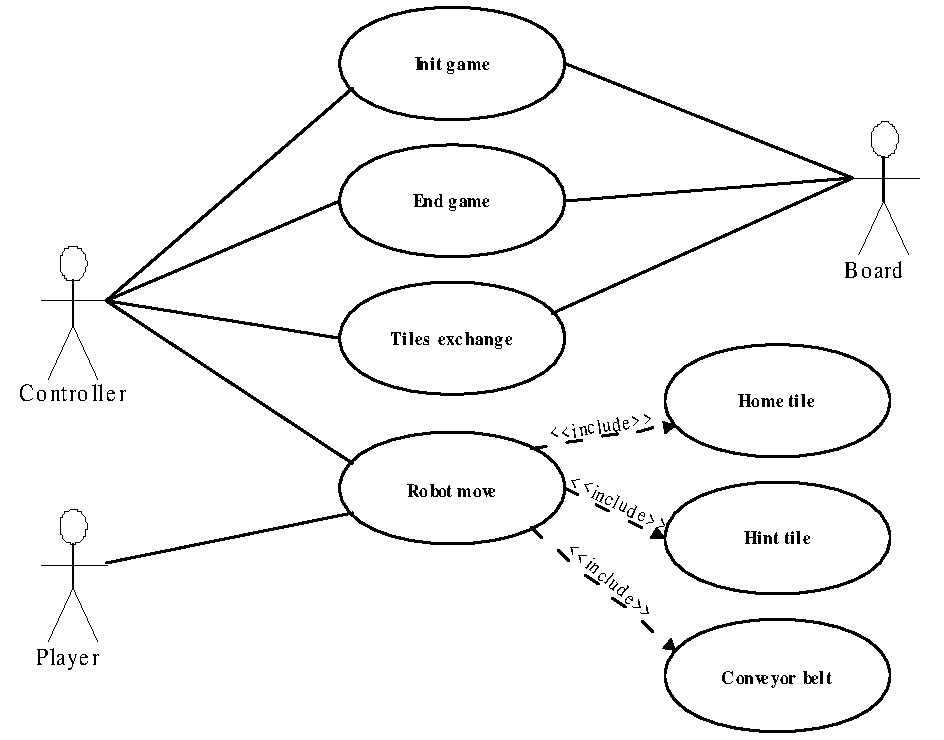
\includegraphics[width=\linewidth]{usecases/diagram.pdf}	

\subsection{High Level Message Sequence Chart}
	The following graph represents our high level message sequence chart and shows how a normal program flow is modeled by MSCs. The graph consists of two parts that run concurrently, the viewer part and the main game part. The viewer part will make sure the viewer updates regularly. The main game part follows the flow of a normal game. 
	
	\digraph[scale=0.4]{HMSC}{
begin2 [label="",shape="invtriangle"];
end2 [label="",shape="triangle"];
initview [label="Initialize viewer",shape="Mrecord"];
updateview [label="Update viewer",shape="Mrecord"];
begin2->initview;
initview->updateview;
updateview->updateview;
updateview->end2;
begin [label="",shape="invtriangle"];
end [label="",shape="triangle"];
p1 [label="",shape="point"];
p2 [label="",shape="point"];
p22 [label="",shape="point"];
p3 [label="",shape="point"];
p4 [label="",shape="point"];
p5 [label="",shape="point"];
p55 [label="",shape="point"];
p6 [label="",shape="point"];
p66 [label="",shape="point"];
p7 [label="",shape="point"];
p77 [label="",shape="point"];
p8 [label="",shape="point"];
init [label="Initialize",shape="Mrecord"];
mvreq [label="Robot move request",shape="Mrecord"];
mvrej [label="Reject move",shape="Mrecord"];
retnt [label="Return Normal tile",shape="Mrecord"];
retht [label="Return Hint tile",shape="Mrecord"];
retct [label="Return Conveyor tile",shape="Mrecord"];
retmt [label="Return Home tile",shape="Mrecord"];
ordex [label="Ordinary exchange",shape="Mrecord"];
spcex [label="Special exchange",shape="Mrecord"];
endgame [label="End game",shape="Mrecord"];
notrob1 [label="Notify robots",shape="Mrecord"];
notrob2 [label="Notify robots",shape="Mrecord"];
begin->p1;
p1->init;
init->p2;
p2->mvreq;
mvreq->p3;
p3->mvrej;
mvrej->p2;
p3->p4;
p4->retnt;
p4->retht;
p4->retct;
p4->retmt;
retnt->p5;
retht->p5;
retct->p5;
p5->p55;
p55->p66;
p66->p6;
p55->notrob1;
notrob1->p66;
p6->ordex;
p6->spcex;
ordex->p7;
spcex->p7;
p7->p77;
p77->p22;
p22->p2 [tailport=e];
p77->notrob2;
notrob2->p22;
retmt->endgame;
endgame->p8;
p8->p1;
p8->end;
}

	%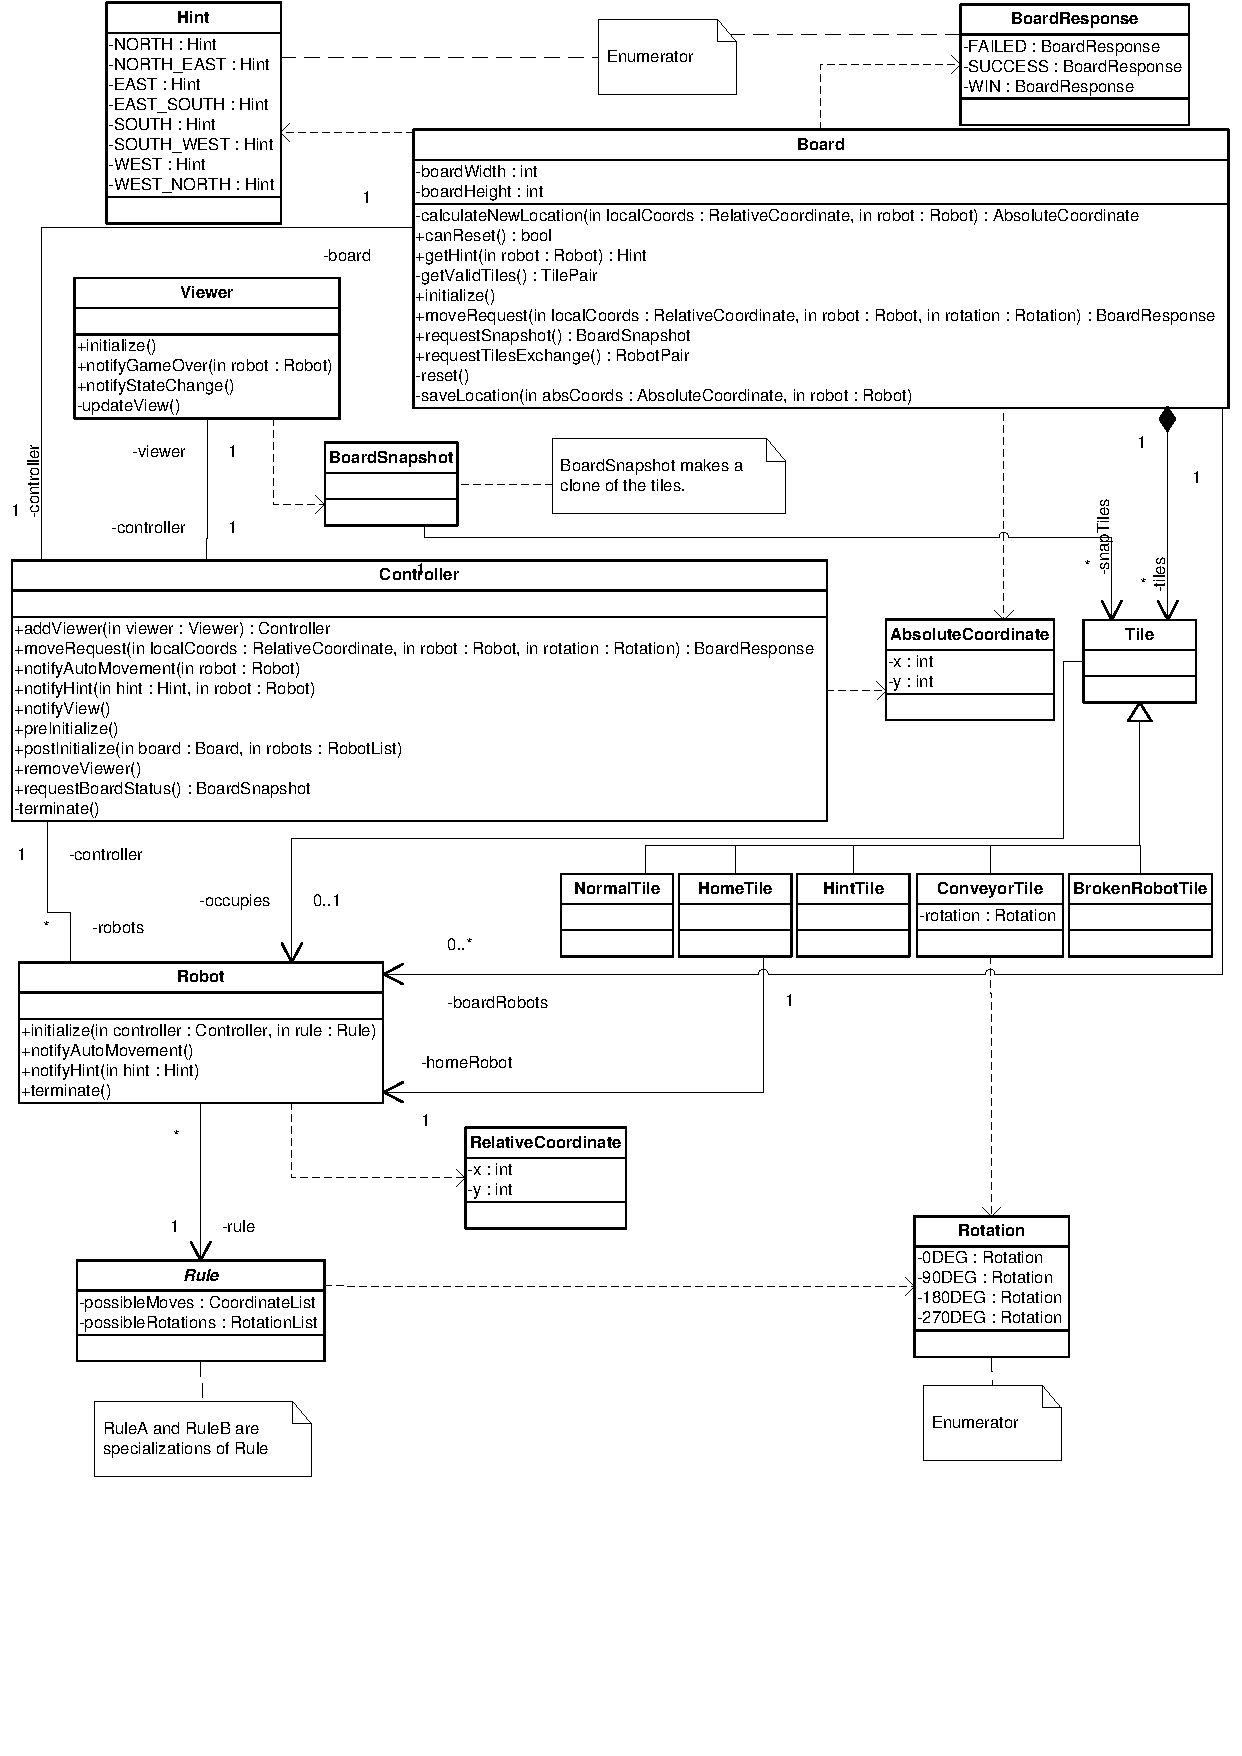
\includegraphics[width=\linewidth]{classdiagram}

\subsection{Message Sequence Charts}
	This section contains the message sequence charts for our use cases. Below every MSC is the location of the MSC in the High Level Message Sequence Chart.

	The world entity is not a real part of our MSCs, but rather a link to the outside world. When an internal action ends in '()' it's a function call to a private function of the entity. Otherwise, it's an action within the called function.

	Note: the symbol $\vdots$ denotes the start and end of a co-region.

	\subsubsection{Initialize viewer}
	The viewer is initialized by the world. Analogous to the HMSC, this happens concurrently to the Initialize MSC.
	
	\begin{msc}
msc
{

w [label="World"],
b [label="Board"],
c [label="Controller"],
v [label="Viewer"];

v box v [label=""],
b box b [label=""],
c box c [label=""],
w box w [label=""];

|||;

w => v [label="initialize(controller)"];
v rbox v [label="initialize"];
v => c [label="addViewer(viewer)"];
c >> v [label="self"];

... [label="board waits a predefined time"];

b rbox b [label="make snapshot"];
b -> c [label="notifyViewer(snapshot)"];
c -> v [label="notifyStateChange(snapshot)"];
v rbox v [label="updateView()"];

|||;

v box v [label="", textbgcolor="black"],
b box b [label="", textbgcolor="black"],
c box c [label="", textbgcolor="black"],
w box w [label="", textbgcolor="black"];

}
\end{msc}
\digraph[scale=0.5]{HMSC_init_view}{rankdir=LR;
p2 [label="",shape="point"];
init [label="Initialize",shape="Mrecord"];
initview [label="Initialize viewer",shape="Mrecord",style=filled];
mvreq [label="Robot move request",shape="Mrecord"];
init->initview;
initview->p2;
p2->mvreq
}


    	\subsubsection{Update viewer}
	During the game execution, the view will keep requesting the current board snapshot from the controller. This happens concurrently to the rest of the process. It can also request the board snapshot when it gets notified by the controller that the board has changed.
    	
	\begin{msc}
msc {

b [label="Board"],
c [label="Controller"],
d [label="Viewer"];

b box b [label=""],
d box d [label=""],
c box c [label=""];

|||;

d => c [label="requestBoardSnapshot()"];
c => b [label="requestBoardStatus()"];
b >> c [label="BoardSnapshot"];
c >> d [label="BoardSnapshot"];
d box d [label="updateView()"];

|||;

d box d [label="", textbgcolor="black"],
c box c [label="", textbgcolor="black"],
b box b [label="", textbgcolor="black"];

}
\end{msc}
\digraph[scale=0.5]{HMSC_upview}{
rankdir=LR;
end2 [label="",shape="triangle"];
initview [label="Initialize viewer",shape="Mrecord"];
updateview [label="Update viewer",shape="Mrecord",style=filled];
initview->updateview;
updateview->updateview;
updateview->end2;
} 

	\subsubsection{Initialize}
	When the game starts, the board is initialized. When this is done, the board sends a preInitialize to the controller. When the controller is done with that, the board will initialize all robots, which will reply with an 'OK' when done. When all robots have been initialized, the board sends a postInitialize to the controller. All entities are now initialized.
  	
	\begin{msc}
msc
{

a [label="Robot"],
b [label="Controller"],
c [label="Board"];

a box a [label=""],
b box b [label=""],
c box c [label=""];

|||;

b rbox b [label="initialize"];

b => a [label="initialize"];
a rbox a [label="initialize"];
a >> b [label=""];

b =>c [label="initialize(robotlist)"];
c rbox c [label="initliaze"];
c >>b [label="OK"];

|||;

a box a [label="", textbgcolor="black"],
b box b [label="", textbgcolor="black"],
c box c [label="", textbgcolor="black"];

}
\end{msc}
\digraph[scale=0.5]{HMSC_init}{rankdir=LR;
begin [label="",shape="invtriangle"];
p1 [label="",shape="point"];
p2 [label="",shape="point"];
init [label="Initialize",shape="Mrecord",style=filled];
mvreq [label="Robot move request",shape="Mrecord"];
begin->p1;
p1->init;
init->p2;
p2->mvreq
}

    	
	\subsubsection{Robot move request}
	A robot can make a move request with the controller, which will forward that to the board. The board will check the validity of the with the robots rule and then check the validity of the move at the current state of the board.

	\begin{msc}
msc
{

d [label="Board"],
c [label="Controller"],
a [label="Robot"],
r [label="Rule"];

d box d [label=""],
c box c [label=""],
a box a [label=""],
r box r [label=""];

|||;

a => c [label="moveRequest(localCoords, robot, rotation)"];
c => d [label="moveRequest(localCoords, robot, rotation)"];
d rbox d [label="get possible moves"], r note r [label="references the robot's ruleset"];
d rbox d [label="get possible rotations"];
d rbox d [label="check if robot can be placed"];

|||;

a box a [label="", textbgcolor="black"],
c box c [label="", textbgcolor="black"],
d box d [label="", textbgcolor="black"],
r box r [label="", textbgcolor="black"];

}
\end{msc}
\digraph[scale=0.5]{HMSC_req}{
rankdir=LR;
p2 [label="",shape="point"];
p3 [label="",shape="point"];
p4 [label="",shape="point"];
init [label="Initialize",shape="Mrecord"];
mvreq [label="Robot move request",shape="Mrecord",style=filled];
mvrej [label="Reject move",shape="Mrecord"];
retnt [label="Return Normal tile",shape="Mrecord"];
retht [label="Return Hint tile",shape="Mrecord"];
retct [label="Return Conveyor tile",shape="Mrecord"];
retmt [label="Return Home tile",shape="Mrecord"];
init->p2;
p2->mvreq;
mvreq->p3;
p3->mvrej;
mvrej->p2;
p3->p4;
p4->retnt;
p4->retht;
p4->retct;
p4->retmt;
}


	\subsubsection{Return Normal tile}
	If the move request is okay, and the robot is moved to a normal tile, the board will return \emph{SUCCESS} to the controller, which will forward this message to the robot that was moved and then notify the viewer that the state of the board has changed.

	\begin{msc}
msc
{

d [label="Board"],
c [label="Controller"],
a [label="Robot"];

d box d [label=""],
c box c [label=""],
a box a [label=""];

|||;

d rbox d [label="calculateNewLocation(localCoords, robot)"];
d rbox d [label="saveLocation(absCoords, robot)"];
d >> c [label="SUCCESS"];
c >> a [label="SUCCESS"];

|||;

a box a [label="", textbgcolor="black"],
c box c [label="", textbgcolor="black"],
d box d [label="", textbgcolor="black"];

}
\end{msc}
\digraph[scale=0.5]{HMSC_mvnt}{
rankdir=LR;
p3 [label="",shape="point"];
p4 [label="",shape="point"];
p5 [label="",shape="point"];
p6 [label="",shape="point"];
notrob1 [label="Notify robots",shape="Mrecord"];
p55 [label="",shape="point"];
p66 [label="",shape="point"];
mvreq [label="Robot move request",shape="Mrecord"];
mvrej [label="Reject move",shape="Mrecord"];
retnt [label="Return Normal tile",shape="Mrecord",style=filled];
ordex [label="Ordinary exchange",shape="Mrecord"];
spcex [label="Special exchange",shape="Mrecord"];
mvreq->p3;
p3->mvrej;
p3->p4;
p4->retnt;
retnt->p5;
p5->p55;
p55->p66;
p66->p6;
p55->notrob1;
notrob1->p66;
p6->ordex;
p6->spcex;
}


	\subsubsection{Return Hint tile}
	If the move request is okay, and the robot is moved to a hint tile, the board will notify the controller that the robot that moved should receive a hint. The controller will notify the viewer that the state of the board has changed and forward the hint to the robot.

	\begin{msc}
msc
{

d [label="Board"],
c [label="Controller"],
a [label="Robot"];

d box d [label=""],
c box c [label=""],
a box a [label=""];

|||;

d rbox d [label="calculateNewLocation(localCoords, robot)"];
d rbox d [label="saveLocation(absCoords, robot)"];
d >> c [label="HINT"];
c => d [label="getHint(robot)"];
d rbox d [label="generate hint"];
d >> c [label="hint"];
c => a [label="notifyHint(hint)"];

|||;

a box a [label="", textbgcolor="black"],
c box c [label="", textbgcolor="black"],
d box d [label="", textbgcolor="black"];

}
\end{msc}
\digraph[scale=0.5]{HMSC_mvht}{
rankdir=LR;
p3 [label="",shape="point"];
p4 [label="",shape="point"];
p5 [label="",shape="point"];
p6 [label="",shape="point"];
mvreq [label="Robot move request",shape="Mrecord"];
mvrej [label="Reject move",shape="Mrecord"];
retht [label="Return Hint tile",shape="Mrecord",style=filled];
ordex [label="Ordinary exchange",shape="Mrecord"];
spcex [label="Special exchange",shape="Mrecord"];
mvreq->p3;
p3->mvrej;
p3->p4;
p4->retht;
retht->p5;
p5->p6;
p6->ordex;
p6->spcex;
}


	\subsubsection{Return Conveyor tile}
	If the move request is okay, and the robot is moved to a conveyor tile, the board will notify the controller that the robot was moved successfully. The controller will notify the viewer that the state of the board is updated and forward the message from the board to the robot. The board will then send a message to the controller that the robot was moved automatically (this was due to the conveyor belt) and the controller will forward this message to the robot.

	\begin{msc}
msc
{

d [label="Board"],
c [label="Controller"],
a [label="Robot"];

d box d [label=""],
c box c [label=""],
a box a [label=""];

|||;

d rbox d [label="calculateNewLocation(localCoords, robot)"];
d rbox d [label="saveLocation(absCoords, robot)"];
d >> c [label="SUCCESS"];
c >> a [label="SUCCESS"];

|||;

d -> c [label="notifyAutoMovement(robot)"];
c -> a [label="notifyAutoMovement()"];


|||;

a box a [label="", textbgcolor="black"],
c box c [label="", textbgcolor="black"],
d box d [label="", textbgcolor="black"];

}
\end{msc}
\digraph[scale=0.5]{HMSC_mvct}{
rankdir=LR;
p3 [label="",shape="point"];
p4 [label="",shape="point"];
p5 [label="",shape="point"];
p6 [label="",shape="point"];
notrob1 [label="Notify robots",shape="Mrecord"];
p55 [label="",shape="point"];
p66 [label="",shape="point"];
mvreq [label="Robot move request",shape="Mrecord"];
mvrej [label="Reject move",shape="Mrecord"];
retct [label="Return Conveyor tile",shape="Mrecord",style=filled];
ordex [label="Ordinary exchange",shape="Mrecord"];
spcex [label="Special exchange",shape="Mrecord"];
mvreq->p3;
p3->mvrej;
p3->p4;
p4->retct;
retct->p5;
p5->p55;
p55->p66;
p66->p6;
p55->notrob1;
notrob1->p66;
p6->ordex;
p6->spcex;
}


	\subsubsection{Return Home tile}
	If the move request is okay, and the robot is moved to its home tile, the board will notify the controller that the robot that moved wins the game. The controller notifies the viewer that the state of the board has changed.

	\begin{msc}
msc
{

a [label="Robot"],
c [label="Controller"],
d [label="Board"];

a box a [label=""],
c box c [label=""],
d box d [label=""];

|||;

d rbox d [label="calculateNewLocation(localCoords, robot)"];
d rbox d [label="saveLocation(absCoords, robot)"];
d >> c [label="WIN"];
c => a [label="terminate"];
a note a [label="each robot, except the robot that won the game, receives a terminate from the controller"];

|||;

a box a [label="", textbgcolor="black"],
c box c [label="", textbgcolor="black"],
d box d [label="", textbgcolor="black"];

}
\end{msc}



	\subsubsection{Reject move}
	If the move request is, for whatever reason, not okay, the board will notify the controller of this. The controller will forward this to the robot that tried to move.

	\begin{msc}
msc
{

a [label="Robot"],
c [label="Controller"],
d [label="Board"],
r [label="Rule"];

a box a [label=""],
c box c [label=""],
d box d [label=""],
r box r [label=""];

|||;

r >> d [label="NOK"];
d >> c [label="NOK"];
c -> a [label="NOK"];

|||;

a box a [label="", textbgcolor="black"],
c box c [label="", textbgcolor="black"],
d box d [label="", textbgcolor="black"],
r box r [label="", textbgcolor="black"];

}
\end{msc}
\digraph[scale=0.5]{HMSC_mvrej}{
rankdir=LR;
p2 [label="",shape="point"];
p3 [label="",shape="point"];
init [label="Initialize",shape="Mrecord"];
mvreq [label="Robot move request",shape="Mrecord"];
mvrej [label="Reject move",shape="Mrecord",style=filled];
init->p2;
p2->mvreq;
mvreq->p3;
p3->mvrej;
mvrej->p2;
}



	\advance\count17 by -6

	\subsubsection{Ordinary exchange}
	The controller requests the board to do a tile exchange. The board will get two valid tiles (internally, this function relies on the rule entities), swap them and returns an empty RobotPair to signal that there were no robots on the tiles.

	\begin{msc}
msc
{

b [label="Board"],
c [label="Controller"];

c box c [label=""],
b box b [label=""];

|||;

c=>b [label="requestTilesExchange()"];
b rbox b [label="exchange two tiles"];
b>>c [label="empty RobotPair"];

|||;

b box b [label="",textbgcolor="black"],
c box c [label="",textbgcolor="black"];

}
\end{msc}
\digraph[scale=0.5]{HMSC_exch}{
rankdir=LR;
p2 [label="",shape="point"];
p5 [label="",shape="point"];
p6 [label="",shape="point"];
p7 [label="",shape="point"];
init [label="Initialize",shape="Mrecord"];
mvreq [label="Robot move request",shape="Mrecord"];
retnt [label="Return Normal tile",shape="Mrecord"];
retht [label="Return Hint tile",shape="Mrecord"];
retct [label="Return Conveyor tile",shape="Mrecord"];
ordex [label="Ordinary exchange",shape="Mrecord",style=filled];
init->p2;
p2->mvreq;
retnt->p5;
retht->p5;
retct->p5;
p5->p6;
p6->ordex;
ordex->p7;
p7->p2;
}


	\subsubsection{Special exchange}
	Like in the ordinary exchange, the controller requests the board to do a tile exchange. The board will find two valid tiles (with on at least one of them a robot or a conveyor belt) and swap them. The board will return a RobotPair with the robots that have been selected in it (so either an empty RobotPair, a RobotPair with one robot, or a RobotPair with two robots). The selected conveyor tiles and robots will be rotated. The controller will notify all players that have been moved and then notify the viewer that the state of the board has changed. Here, one robot and one conveyor belt have been selected.

	\begin{msc}
msc
{

b [label="Board"],
c [label="Controller"],
p1 [label="Robot1"],
p2 [label="Robot2"],
v [label="Viewer"];

c box c [label=""],
b box b [label=""],
p1 box p1 [label=""],
p2 box p2 [label=""],
v box v [label=""];

|||;
c=>b [label="requestTilesExchange()"];
b rbox b [label="getValidTiles()"];
b rbox b [label="exchange two valid tiles"];
b rbox b [label="rotate robot1 and rotate tiles"];
b>>c [label="RobotPair with one robot"];
...;
c->p1 [label="notifyAutoMovement()"];
c -> v [label="notifyStateChange()"];
...;

|||;

b box b [label="",textbgcolor="black"],
c box c [label="",textbgcolor="black"],
p1 box p1 [label="",textbgcolor="black"],
p2 box p2 [label="",textbgcolor="black"],
v box v [label="",textbgcolor="black"];

}
\end{msc}

\digraph[scale=0.5]{HMSC_exchsp}{
rankdir=LR;
p2 [label="",shape="point"];
p5 [label="",shape="point"];
p6 [label="",shape="point"];
p7 [label="",shape="point"];
p22 [label="",shape="point"];
p77 [label="",shape="point"];
notrob2 [label="Notify robots",shape="Mrecord"];
init [label="Initialize",shape="Mrecord"];
mvreq [label="Robot move request",shape="Mrecord"];
retnt [label="Return Normal tile",shape="Mrecord"];
retht [label="Return Hint tile",shape="Mrecord"];
retct [label="Return Conveyor tile",shape="Mrecord"];
spcex [label="Special exchange",shape="Mrecord",style=filled];
init->p2;
p2->mvreq;
retnt->p5;
retht->p5;
retct->p5;
p5->p6;
p6->spcex;
spcex->p7;
p7->p77;
p77->p22;
p22->p2;
p77->notrob2;
notrob2->p22;
}

	
	\subsubsection{Notify robots}
	The board sends a notification to the controller, which forwards this to the robot that was moved.	

	The notify robots MSC will be inserted here.


	\subsubsection{End game}
	The controller will send a terminate message to all losing robots, which will then terminate safely. The controller will then notify the view which robot won the game, so it can show to end game animation. When the animation is done, the call will return and the controller will send a message to the board that everything it done and the board can reset and will then terminate. The winning robot will also terminate. The board can then choose to either reset to start a new game or terminate.

	\begin{msc}
msc
{

b [label="Board"],
c [label="Controller"],
p [label="Robot"],
v [label="View"];

b box b [label=""],
c box c [label=""],
p box p [label=""],
v box v [label=""];

|||;

c -> p [label="terminate"];
p rbox p [label="terminate()"];
p note p [label="From here on, robot is the robot that has won the game"];
c -> v [label="notifyGameOver(robot)"];
v rbox v [label="fireworks"];
v >> c [label="done"];
c -> b [label="canReset"];
v rbox v [label="terminate"],
b rbox b [label="reset()"],
c rbox c [label="terminate()"];


|||;

b box b [label="",textbgcolor="black"],
c box c [label="",textbgcolor="black"],
p box p [label="",textbgcolor="black"],
v box v [label="",textbgcolor="black"];

}
\end{msc}
\digraph[scale=0.5]{HMSC_end}{
rankdir=LR;
begin [label="",shape="invtriangle"];
end [label="",shape="triangle"];
p1 [label="",shape="point"];
p8 [label="",shape="point"];
init [label="Initialize",shape="Mrecord"];
retmt [label="Return Home tile",shape="Mrecord"];
endgame [label="End game",shape="Mrecord",style=filled];
begin->p1;
p1->init;
retmt->endgame;
endgame->p8;
p8->p1;
p8->end;
}


	\newpage

	\section{Message sequence charts}
	This section contains the message sequence charts, both of high and class level.
\subsection{High Level Message Sequence Chart}
	
	\begin{minipage}{\linewidth}
		The following graph represents our high level message sequence chart and shows how a normal program flow is modeled by MSCs.
		
		\digraph[scale=0.4]{HMSC}{
begin2 [label="",shape="invtriangle"];
end2 [label="",shape="triangle"];
initview [label="Initialize viewer",shape="Mrecord"];
updateview [label="Update viewer",shape="Mrecord"];
begin2->initview;
initview->updateview;
updateview->updateview;
updateview->end2;
begin [label="",shape="invtriangle"];
end [label="",shape="triangle"];
p1 [label="",shape="point"];
p2 [label="",shape="point"];
p22 [label="",shape="point"];
p3 [label="",shape="point"];
p4 [label="",shape="point"];
p5 [label="",shape="point"];
p55 [label="",shape="point"];
p6 [label="",shape="point"];
p66 [label="",shape="point"];
p7 [label="",shape="point"];
p77 [label="",shape="point"];
p8 [label="",shape="point"];
init [label="Initialize",shape="Mrecord"];
mvreq [label="Robot move request",shape="Mrecord"];
mvrej [label="Reject move",shape="Mrecord"];
retnt [label="Return Normal tile",shape="Mrecord"];
retht [label="Return Hint tile",shape="Mrecord"];
retct [label="Return Conveyor tile",shape="Mrecord"];
retmt [label="Return Home tile",shape="Mrecord"];
ordex [label="Ordinary exchange",shape="Mrecord"];
spcex [label="Special exchange",shape="Mrecord"];
endgame [label="End game",shape="Mrecord"];
notrob1 [label="Notify robots",shape="Mrecord"];
notrob2 [label="Notify robots",shape="Mrecord"];
begin->p1;
p1->init;
init->p2;
p2->mvreq;
mvreq->p3;
p3->mvrej;
mvrej->p2;
p3->p4;
p4->retnt;
p4->retht;
p4->retct;
p4->retmt;
retnt->p5;
retht->p5;
retct->p5;
p5->p55;
p55->p66;
p66->p6;
p55->notrob1;
notrob1->p66;
p6->ordex;
p6->spcex;
ordex->p7;
spcex->p7;
p7->p77;
p77->p22;
p22->p2 [tailport=e];
p77->notrob2;
notrob2->p22;
retmt->endgame;
endgame->p8;
p8->p1;
p8->end;
}
	
	\end{minipage}
	\newpage
\subsection{Message Sequence Charts}
	This section contains the message sequence charts for our use cases. Below every MSC is the location of the MSC in the High Level Message Sequence Chart, which shows the possible routes that can be taken from the corresponding MSC. For example, below the MSC 'Initialize', both 'Initialize' and 'Move Request' are shown, since 'Move Request' is the next step after 'Initialize' has been completed. If several options for next moves exist, they are given in the same way as in the HMSC below; in the corresponding separate MSC is explained when and why a certain route is taken. Note that the below MSCs are identical to the use cases described in section 1.

	The world entity is not a real part of our MSCs, but rather a link to the outside world. When an internal action is postfixed with '()' it's a function call to a private function of the entity. Otherwise, it is an action within the called function.

	The following MSC syntax is used in this section:

	\begin{msc}
	msc{
        	a, b;

        	a -> b [label="A signal"];
        	a => b [label="A function call"];
        	b >> a [label="A return value"];
        	b rbox b [label="An internal action"];

	}
\end{msc}


	\subsubsection{Initialize}
	\begin{minipage}{\linewidth}
		When the game starts, the board is initialized. When this is done, the board sends a preInitialize to the controller. When the controller is done with that, the board will initialize all robots (choosing the appropriate rule for them), which will reply with an 'OK' when done. When all robots have been initialized, the board sends a postInitialize to the controller. All entities are now initialized. \\
		Separate pre- and post-initialize method are used because the controller can not fully initialize without the robots and the robots, in turn, must be initialized with the controller. So, the pre-initialize is used to create the controller and the post-initialize is used to store all the robots that have been initialized by the board.

		\begin{msc}
msc
{

a [label="Robot"],
b [label="Controller"],
c [label="Board"];

a box a [label=""],
b box b [label=""],
c box c [label=""];

|||;

b rbox b [label="initialize"];

b => a [label="initialize"];
a rbox a [label="initialize"];
a >> b [label=""];

b =>c [label="initialize(robotlist)"];
c rbox c [label="initliaze"];
c >>b [label="OK"];

|||;

a box a [label="", textbgcolor="black"],
b box b [label="", textbgcolor="black"],
c box c [label="", textbgcolor="black"];

}
\end{msc}
\digraph[scale=0.5]{HMSC_init}{rankdir=LR;
begin [label="",shape="invtriangle"];
p1 [label="",shape="point"];
p2 [label="",shape="point"];
init [label="Initialize",shape="Mrecord",style=filled];
mvreq [label="Robot move request",shape="Mrecord"];
begin->p1;
p1->init;
init->p2;
p2->mvreq
}

    \end{minipage}

    \subsubsection{Initialize viewer}
	\begin{minipage}{\linewidth}
		The viewer is initialized by the world. Note that the world provides a parameter 'controller' to the viewer, so the viewer knows how to address the controller. Analogous to the HMSC, this happens after the components of the game (board, controller, etcetera) have been initialized. After the call has been received, the viewer will initialize itself and will attach itself to the controller, via addViewer. Once the viewer has been succesfully attached, the controller returns itself to notify the viewer of this success.
	
		\begin{msc}
msc
{

w [label="World"],
b [label="Board"],
c [label="Controller"],
v [label="Viewer"];

v box v [label=""],
b box b [label=""],
c box c [label=""],
w box w [label=""];

|||;

w => v [label="initialize(controller)"];
v rbox v [label="initialize"];
v => c [label="addViewer(viewer)"];
c >> v [label="self"];

... [label="board waits a predefined time"];

b rbox b [label="make snapshot"];
b -> c [label="notifyViewer(snapshot)"];
c -> v [label="notifyStateChange(snapshot)"];
v rbox v [label="updateView()"];

|||;

v box v [label="", textbgcolor="black"],
b box b [label="", textbgcolor="black"],
c box c [label="", textbgcolor="black"],
w box w [label="", textbgcolor="black"];

}
\end{msc}
\digraph[scale=0.5]{HMSC_init_view}{rankdir=LR;
p2 [label="",shape="point"];
init [label="Initialize",shape="Mrecord"];
initview [label="Initialize viewer",shape="Mrecord",style=filled];
mvreq [label="Robot move request",shape="Mrecord"];
init->initview;
initview->p2;
p2->mvreq
}

	\end{minipage}

	\subsubsection{Robot move request}
	\begin{minipage}{\linewidth}
		A robot can make a move request with the controller, which will forward that to the board. The board will check the validity of the move itself with the robots rule and then check the validity of the move at the current state of the board. The internal actions 'get possible moves' and 'get possible rotations' are thus used by the board to check whether the move request is conform with the specified moves and rotations in the rule of the robot. Based upon the outcome of the move request, one of the five MSCs given in the HMSC below is executed. \\
		Note that the move requests describe a move request in terms of local coordinates, since a robot does not know its exact location on the board. Also, the move request contains the robot that requested the move, along with the requested rotation.

		\begin{msc}
msc
{

d [label="Board"],
c [label="Controller"],
a [label="Robot"],
r [label="Rule"];

d box d [label=""],
c box c [label=""],
a box a [label=""],
r box r [label=""];

|||;

a => c [label="moveRequest(localCoords, robot, rotation)"];
c => d [label="moveRequest(localCoords, robot, rotation)"];
d rbox d [label="get possible moves"], r note r [label="references the robot's ruleset"];
d rbox d [label="get possible rotations"];
d rbox d [label="check if robot can be placed"];

|||;

a box a [label="", textbgcolor="black"],
c box c [label="", textbgcolor="black"],
d box d [label="", textbgcolor="black"],
r box r [label="", textbgcolor="black"];

}
\end{msc}
\digraph[scale=0.5]{HMSC_req}{
rankdir=LR;
p2 [label="",shape="point"];
p3 [label="",shape="point"];
p4 [label="",shape="point"];
init [label="Initialize",shape="Mrecord"];
mvreq [label="Robot move request",shape="Mrecord",style=filled];
mvrej [label="Reject move",shape="Mrecord"];
retnt [label="Return Normal tile",shape="Mrecord"];
retht [label="Return Hint tile",shape="Mrecord"];
retct [label="Return Conveyor tile",shape="Mrecord"];
retmt [label="Return Home tile",shape="Mrecord"];
init->p2;
p2->mvreq;
mvreq->p3;
p3->mvrej;
mvrej->p2;
p3->p4;
p4->retnt;
p4->retht;
p4->retct;
p4->retmt;
}

    \end{minipage}

	\subsubsection{Return Normal tile}
	\begin{minipage}{\linewidth}
		If the move request is valid, and the robot is moved to a normal tile, the board will return \emph{SUCCESS} to the controller, which will forward this message to the robot that was moved. Internally, the board calculates the new location of the robot and saves the location if the move request is valid.

		\begin{msc}
msc
{

d [label="Board"],
c [label="Controller"],
a [label="Robot"];

d box d [label=""],
c box c [label=""],
a box a [label=""];

|||;

d rbox d [label="calculateNewLocation(localCoords, robot)"];
d rbox d [label="saveLocation(absCoords, robot)"];
d >> c [label="SUCCESS"];
c >> a [label="SUCCESS"];

|||;

a box a [label="", textbgcolor="black"],
c box c [label="", textbgcolor="black"],
d box d [label="", textbgcolor="black"];

}
\end{msc}
\digraph[scale=0.5]{HMSC_mvnt}{
rankdir=LR;
p3 [label="",shape="point"];
p4 [label="",shape="point"];
p5 [label="",shape="point"];
p6 [label="",shape="point"];
notrob1 [label="Notify robots",shape="Mrecord"];
p55 [label="",shape="point"];
p66 [label="",shape="point"];
mvreq [label="Robot move request",shape="Mrecord"];
mvrej [label="Reject move",shape="Mrecord"];
retnt [label="Return Normal tile",shape="Mrecord",style=filled];
ordex [label="Ordinary exchange",shape="Mrecord"];
spcex [label="Special exchange",shape="Mrecord"];
mvreq->p3;
p3->mvrej;
p3->p4;
p4->retnt;
retnt->p5;
p5->p55;
p55->p66;
p66->p6;
p55->notrob1;
notrob1->p66;
p6->ordex;
p6->spcex;
}

	\end{minipage}

	\subsubsection{Return Hint tile}
	\begin{minipage}{\linewidth}
		If the move request is valid, and the robot is moved to a hint tile, the board will first respond with \emph{SUCCESS}, to indicate that the move request has been granted. Hereafter, the board generates a hint then notifies the controller that the robot that moved should receive a hint; the controller will forward the hint to the robot. Note that the notifyHint from the board to the controller also contains a robot, since the controller must be able to identify the robot that should receive the hint.

		\begin{msc}
msc
{

d [label="Board"],
c [label="Controller"],
a [label="Robot"];

d box d [label=""],
c box c [label=""],
a box a [label=""];

|||;

d rbox d [label="calculateNewLocation(localCoords, robot)"];
d rbox d [label="saveLocation(absCoords, robot)"];
d >> c [label="HINT"];
c => d [label="getHint(robot)"];
d rbox d [label="generate hint"];
d >> c [label="hint"];
c => a [label="notifyHint(hint)"];

|||;

a box a [label="", textbgcolor="black"],
c box c [label="", textbgcolor="black"],
d box d [label="", textbgcolor="black"];

}
\end{msc}
\digraph[scale=0.5]{HMSC_mvht}{
rankdir=LR;
p3 [label="",shape="point"];
p4 [label="",shape="point"];
p5 [label="",shape="point"];
p6 [label="",shape="point"];
mvreq [label="Robot move request",shape="Mrecord"];
mvrej [label="Reject move",shape="Mrecord"];
retht [label="Return Hint tile",shape="Mrecord",style=filled];
ordex [label="Ordinary exchange",shape="Mrecord"];
spcex [label="Special exchange",shape="Mrecord"];
mvreq->p3;
p3->mvrej;
p3->p4;
p4->retht;
retht->p5;
p5->p6;
p6->ordex;
p6->spcex;
}

	\end{minipage}

	\subsubsection{Return Conveyor tile}
	\begin{minipage}{\linewidth}
		If the move request is valid, and the robot is moved to a conveyor tile, the board again returns \emph{SUCCESS} to the controller, which forwards this message to the robot that was moved. The board will then notify the controller that the robot was moved successfully and the controller will forward this to the robot. The board will then send a message to the controller that the robot was moved automatically (this was due to the conveyor belt) and the controller will forward this message to the robot, using notifyAutoMovement. As in the 'Return Hint tile' MSC, the notifyAutoMovement from the board to the controller contains the robot that should be notified.

		\begin{msc}
msc
{

d [label="Board"],
c [label="Controller"],
a [label="Robot"];

d box d [label=""],
c box c [label=""],
a box a [label=""];

|||;

d rbox d [label="calculateNewLocation(localCoords, robot)"];
d rbox d [label="saveLocation(absCoords, robot)"];
d >> c [label="SUCCESS"];
c >> a [label="SUCCESS"];

|||;

d -> c [label="notifyAutoMovement(robot)"];
c -> a [label="notifyAutoMovement()"];


|||;

a box a [label="", textbgcolor="black"],
c box c [label="", textbgcolor="black"],
d box d [label="", textbgcolor="black"];

}
\end{msc}
\digraph[scale=0.5]{HMSC_mvct}{
rankdir=LR;
p3 [label="",shape="point"];
p4 [label="",shape="point"];
p5 [label="",shape="point"];
p6 [label="",shape="point"];
notrob1 [label="Notify robots",shape="Mrecord"];
p55 [label="",shape="point"];
p66 [label="",shape="point"];
mvreq [label="Robot move request",shape="Mrecord"];
mvrej [label="Reject move",shape="Mrecord"];
retct [label="Return Conveyor tile",shape="Mrecord",style=filled];
ordex [label="Ordinary exchange",shape="Mrecord"];
spcex [label="Special exchange",shape="Mrecord"];
mvreq->p3;
p3->mvrej;
p3->p4;
p4->retct;
retct->p5;
p5->p55;
p55->p66;
p66->p6;
p55->notrob1;
notrob1->p66;
p6->ordex;
p6->spcex;
}

	\end{minipage}

	\subsubsection{Return Home tile}
	\begin{minipage}{\linewidth}
	   If the move request is valid, and the robot is moved to its home tile, the board will notify the controller that the robot that moved wins the game, using the response \emph{WIN}.

		\begin{msc}
msc
{

a [label="Robot"],
c [label="Controller"],
d [label="Board"];

a box a [label=""],
c box c [label=""],
d box d [label=""];

|||;

d rbox d [label="calculateNewLocation(localCoords, robot)"];
d rbox d [label="saveLocation(absCoords, robot)"];
d >> c [label="WIN"];
c => a [label="terminate"];
a note a [label="each robot, except the robot that won the game, receives a terminate from the controller"];

|||;

a box a [label="", textbgcolor="black"],
c box c [label="", textbgcolor="black"],
d box d [label="", textbgcolor="black"];

}
\end{msc}

	\end{minipage}

	\subsubsection{Reject move}
	\begin{minipage}{\linewidth}
		If the move request is, for whatever reason, not valid, the board will notify the controller of this, using the response \emph{FAILED}. The controller will forward this to the robot that made the move request.

		\begin{msc}
msc
{

a [label="Robot"],
c [label="Controller"],
d [label="Board"],
r [label="Rule"];

a box a [label=""],
c box c [label=""],
d box d [label=""],
r box r [label=""];

|||;

r >> d [label="NOK"];
d >> c [label="NOK"];
c -> a [label="NOK"];

|||;

a box a [label="", textbgcolor="black"],
c box c [label="", textbgcolor="black"],
d box d [label="", textbgcolor="black"],
r box r [label="", textbgcolor="black"];

}
\end{msc}
\digraph[scale=0.5]{HMSC_mvrej}{
rankdir=LR;
p2 [label="",shape="point"];
p3 [label="",shape="point"];
init [label="Initialize",shape="Mrecord"];
mvreq [label="Robot move request",shape="Mrecord"];
mvrej [label="Reject move",shape="Mrecord",style=filled];
init->p2;
p2->mvreq;
mvreq->p3;
p3->mvrej;
mvrej->p2;
}

	\end{minipage}

	\advance\count17 by -6

    \subsubsection{Update viewer}
	\begin{minipage}{\linewidth}
        Whenever the board has changed, either because of a move request or a tiles exchange, the board prepares a snapshot for the viewer.	The board notifies the controller that it has a new snapshot for the viewer, using notifyViewer. The controller will then notify the viewer and send the board snapshot, using notifyStateChange; the viewer will internally update its view.

		\begin{msc}
msc {

b [label="Board"],
c [label="Controller"],
d [label="Viewer"];

b box b [label=""],
d box d [label=""],
c box c [label=""];

|||;

d => c [label="requestBoardSnapshot()"];
c => b [label="requestBoardStatus()"];
b >> c [label="BoardSnapshot"];
c >> d [label="BoardSnapshot"];
d box d [label="updateView()"];

|||;

d box d [label="", textbgcolor="black"],
c box c [label="", textbgcolor="black"],
b box b [label="", textbgcolor="black"];

}
\end{msc}
\digraph[scale=0.5]{HMSC_upview}{
rankdir=LR;
end2 [label="",shape="triangle"];
initview [label="Initialize viewer",shape="Mrecord"];
updateview [label="Update viewer",shape="Mrecord",style=filled];
initview->updateview;
updateview->updateview;
updateview->end2;
} 
	\end{minipage}

	\subsubsection{Ordinary exchange}
	\begin{minipage}{\linewidth}
		The controller requests the board to do a tile exchange. The board will get two valid tiles, swap them and inform the controller that the tiles exchange was successful. Note that the 'getValidTiles'-function must maintain the "always reachable home tile"-invariant: each robot must always be able to reach its home tile. The board will calculate this internally and selects two valid tiles without robots in this case.

		\begin{msc}
msc
{

b [label="Board"],
c [label="Controller"];

c box c [label=""],
b box b [label=""];

|||;

c=>b [label="requestTilesExchange()"];
b rbox b [label="exchange two tiles"];
b>>c [label="empty RobotPair"];

|||;

b box b [label="",textbgcolor="black"],
c box c [label="",textbgcolor="black"];

}
\end{msc}
\digraph[scale=0.5]{HMSC_exch}{
rankdir=LR;
p2 [label="",shape="point"];
p5 [label="",shape="point"];
p6 [label="",shape="point"];
p7 [label="",shape="point"];
init [label="Initialize",shape="Mrecord"];
mvreq [label="Robot move request",shape="Mrecord"];
retnt [label="Return Normal tile",shape="Mrecord"];
retht [label="Return Hint tile",shape="Mrecord"];
retct [label="Return Conveyor tile",shape="Mrecord"];
ordex [label="Ordinary exchange",shape="Mrecord",style=filled];
init->p2;
p2->mvreq;
retnt->p5;
retht->p5;
retct->p5;
p5->p6;
p6->ordex;
ordex->p7;
p7->p2;
}

	\end{minipage}

	\subsubsection{Special exchange}
	\begin{minipage}{\linewidth}
		As in the ordinary exchange, the controller requests the board to do a tile exchange. The board will find two valid tiles, in this case with on at least one of them a robot or a conveyor belt, and swap them. The selected conveyor tiles and robots will be rotated. Once the tiles exchange is complete, the board will inform the controller. If one or two robots were part of the tiles exchange, the board will inform the controller of this; the controller will then inform the appropriate robots that they have been automoved, because of the exchange. \\
In the MSC below, one robot and one conveyor belt have been selected. Note that robot2 will not be notified, since it was not part of the tiles exchange. As in the MSC 'Ordinary exchange', the board must (internally) make sure that the "always reachable home tile"-invariant is maintained.

		\begin{msc}
msc
{

b [label="Board"],
c [label="Controller"],
p1 [label="Robot1"],
p2 [label="Robot2"],
v [label="Viewer"];

c box c [label=""],
b box b [label=""],
p1 box p1 [label=""],
p2 box p2 [label=""],
v box v [label=""];

|||;
c=>b [label="requestTilesExchange()"];
b rbox b [label="getValidTiles()"];
b rbox b [label="exchange two valid tiles"];
b rbox b [label="rotate robot1 and rotate tiles"];
b>>c [label="RobotPair with one robot"];
...;
c->p1 [label="notifyAutoMovement()"];
c -> v [label="notifyStateChange()"];
...;

|||;

b box b [label="",textbgcolor="black"],
c box c [label="",textbgcolor="black"],
p1 box p1 [label="",textbgcolor="black"],
p2 box p2 [label="",textbgcolor="black"],
v box v [label="",textbgcolor="black"];

}
\end{msc}

\digraph[scale=0.5]{HMSC_exchsp}{
rankdir=LR;
p2 [label="",shape="point"];
p5 [label="",shape="point"];
p6 [label="",shape="point"];
p7 [label="",shape="point"];
p22 [label="",shape="point"];
p77 [label="",shape="point"];
notrob2 [label="Notify robots",shape="Mrecord"];
init [label="Initialize",shape="Mrecord"];
mvreq [label="Robot move request",shape="Mrecord"];
retnt [label="Return Normal tile",shape="Mrecord"];
retht [label="Return Hint tile",shape="Mrecord"];
retct [label="Return Conveyor tile",shape="Mrecord"];
spcex [label="Special exchange",shape="Mrecord",style=filled];
init->p2;
p2->mvreq;
retnt->p5;
retht->p5;
retct->p5;
p5->p6;
p6->spcex;
spcex->p7;
p7->p77;
p77->p22;
p22->p2;
p77->notrob2;
notrob2->p22;
}

	\end{minipage}	

	\subsubsection{Notify robots}
	\begin{minipage}{\linewidth}
		The board first checks recursively for robots that are affected by the original move request. Then, the board sends a notification to the controller, which forwards this to the robot that was moved. This MSC is used when a robot is moved due to the move of another robot, for example when a robot that blocked the end of a conveyor belt moves away and the last robot on the belt should move to the end.
		Note that is it possible for a robot to end up on its home tile like this. Because of this, a BoardResponse is sent back, to indicate a winning (or of course normal) automove.

		The notify robots MSC will be inserted here.

	\end{minipage}

	\subsubsection{End game}
	\begin{minipage}{\linewidth}
		If a robot has reached its home tile, the controller will send a terminate message to all losing robots, which will then terminate safely. The controller will then notify the viewer which robot won the game, so it can show the end game animation. When the animation is done, the viewer detaches itself from the controller, using removeViewer. The controller will then send a message to the board that everything it done and the board can reset and will then terminate. Note that the winning robot can terminate on its own, since its termination does not affect the other components of the game; the viewer can show an appropriate animation that reflects which robot has won. The board can then choose to either reset to start a new game or terminate; since this is a non-deterministic choice from the board, this is not modeled in the MSC below.

		\begin{msc}
msc
{

b [label="Board"],
c [label="Controller"],
p [label="Robot"],
v [label="View"];

b box b [label=""],
c box c [label=""],
p box p [label=""],
v box v [label=""];

|||;

c -> p [label="terminate"];
p rbox p [label="terminate()"];
p note p [label="From here on, robot is the robot that has won the game"];
c -> v [label="notifyGameOver(robot)"];
v rbox v [label="fireworks"];
v >> c [label="done"];
c -> b [label="canReset"];
v rbox v [label="terminate"],
b rbox b [label="reset()"],
c rbox c [label="terminate()"];


|||;

b box b [label="",textbgcolor="black"],
c box c [label="",textbgcolor="black"],
p box p [label="",textbgcolor="black"],
v box v [label="",textbgcolor="black"];

}
\end{msc}
\digraph[scale=0.5]{HMSC_end}{
rankdir=LR;
begin [label="",shape="invtriangle"];
end [label="",shape="triangle"];
p1 [label="",shape="point"];
p8 [label="",shape="point"];
init [label="Initialize",shape="Mrecord"];
retmt [label="Return Home tile",shape="Mrecord"];
endgame [label="End game",shape="Mrecord",style=filled];
begin->p1;
p1->init;
retmt->endgame;
endgame->p8;
p8->p1;
p8->end;
}

	\end{minipage}

	\newpage

	\section{Design}
	\subsection{Class diagram}
	The following graphic is the class diagram that will be used for the specification and the implementation. Note that, for the sake of readability, names of parameters in methods are abbreviated. For instance, the parameter 'loc' in the moveRequest of Board is in the MSCs referred to as 'localCoords', whereas in the class diagram it is abbreviated.

	%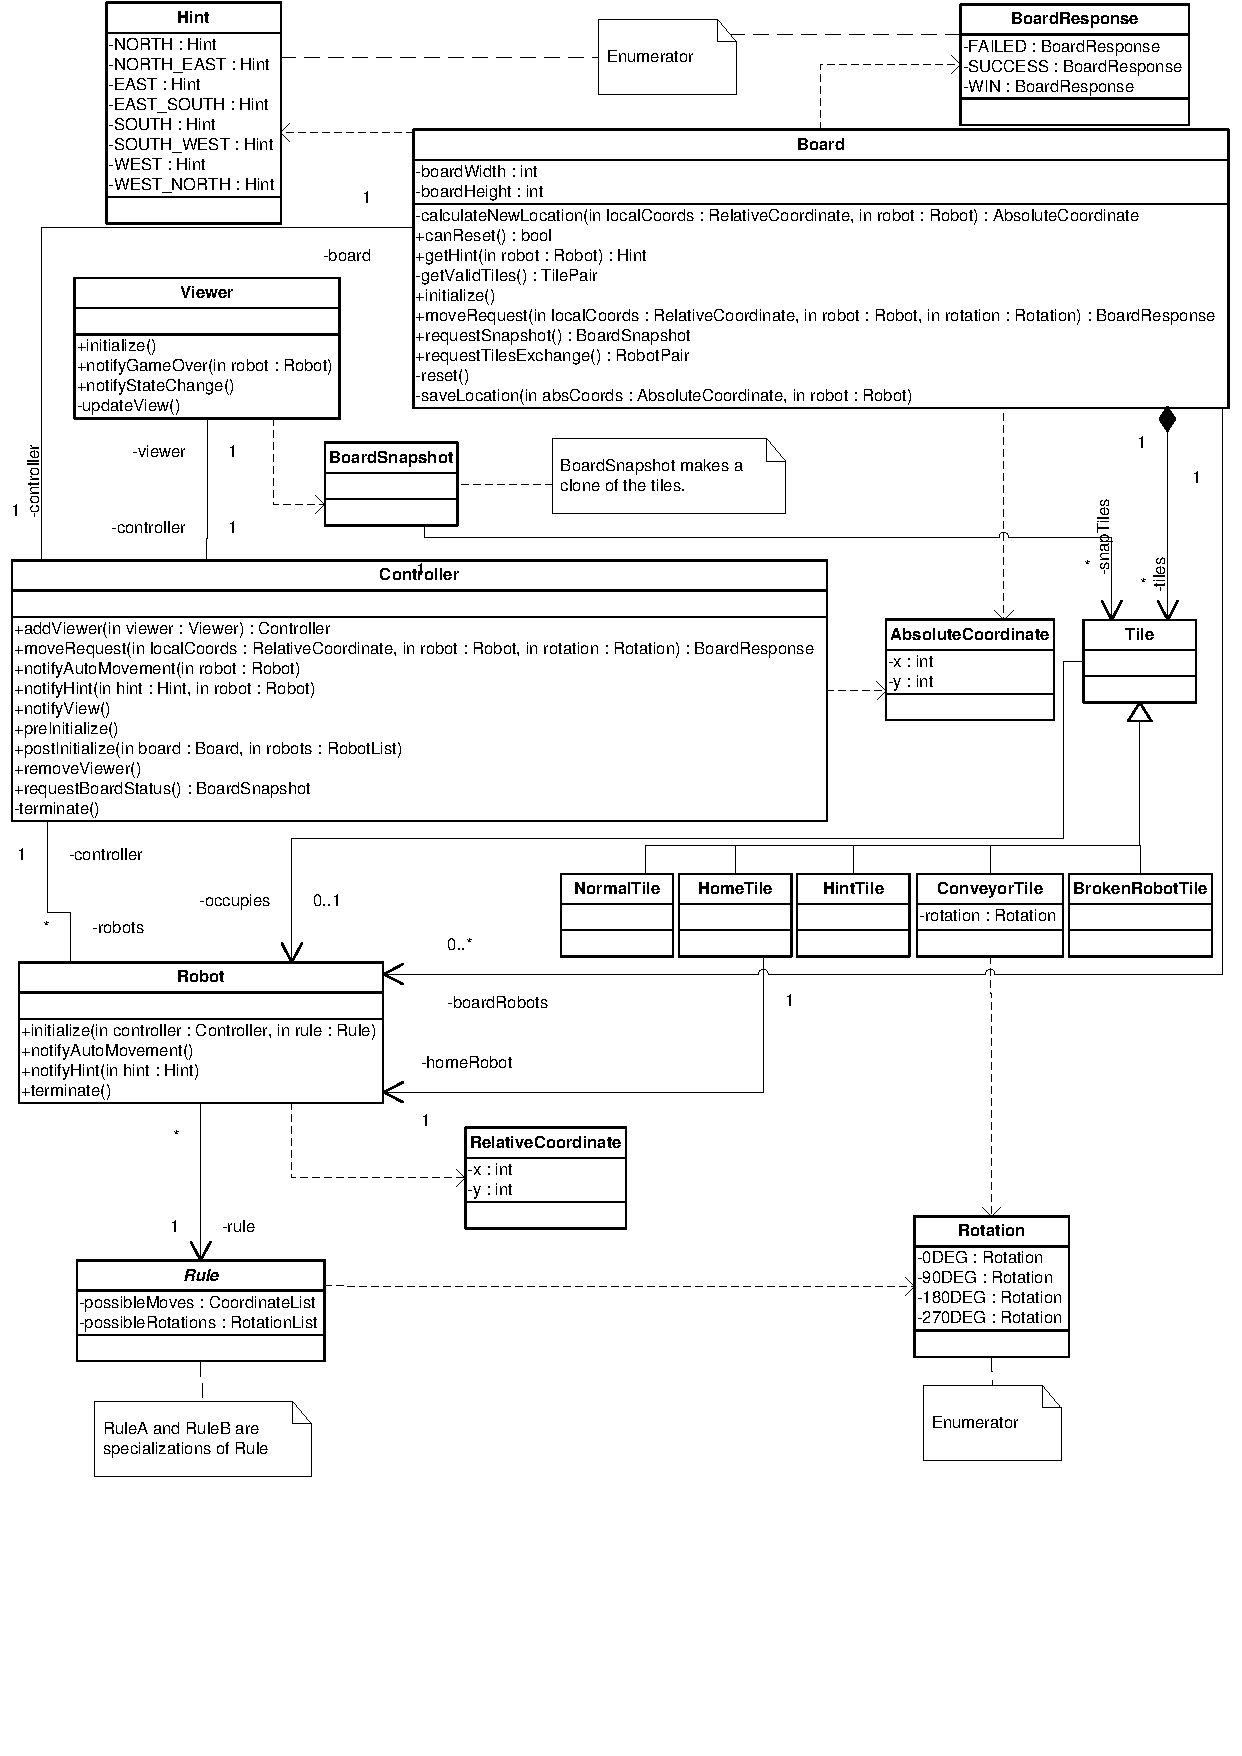
\includegraphics[width=\linewidth]{classdiagram.pdf}
	\let\l=\relax
\let\<=\relax
\let\>=\relax
\digraph[scale=.5]{classdiagram}{
margin=0
fontsize=8
fontname=Helvetica
compound=true
splines=ortho
node [fontsize=8, fontname=Helvetica, shape=record]
edge [fontsize=8, fontname=Helvetica, arrowhead=open, labeldistance=2]
Board [label="{Board|- width : int\l- height : int\l|+ canReset() : bool\l+ initialize()\l+ moveRequest(loc : RelativeCoord, r : Robot, rot : Rotation) : BoardResponse\l+ requestSnapshot() : BoardSnapshot\l+ requestTilesExchange() : bool\l- getHint(r : Robot) : Hint\l- calculateNewLocation(loc : RelativeCoord, r : Robot) :
AbsoluteCoord\l- getValidTiles() : TilePair\l- reset()\l- saveLocation(loc : AbsoluteCoord, r : Robot)\l}"]
Hint [label="{[Hint]| NORTH\l NORTH_EAST\l EAST\l SOUTH_EAST\l SOUTH\l SOUTH_WEST\l WEST\l NORTH_WEST\l}"]
BoardResponse [label="{[BoardResponse]| FAILED\l SUCCESS\l WIN\l}"]
Viewer [label="{Viewer||+ initialize()\l+ notifyGameOver(r : Robot)\l+ notifyStateChange()\l- updateView()\l}"]
BoardSnapshot [label="{BoardSnapshot||}"]
Controller [label="{Controller||+ addViewer(v : Viewer) : Controller\l+ moveRequest(loc : RelativeCoord, r : Robot, rot : Rotation) : BoardResponse\l+ notifyAutoMovement(r : Robot)\l+ notifyHint(h : Hint, r : Robot)\l+ notifyView()\l+ preInitialize()\l+ postInitialize(b : Board, rs : RobotList)\l+ removeViewer()\l+ requestBoardSnapshot() : BoardSnapshot\l- terminate()\l}"]
AbsoluteCoord [label="{AbsoluteCoord|+ x : int\l+ y : int\l|}"]
Tile [label="{Tile||}"]
/**/
subgraph cluster_Tiles {
NormalTile [label="{NormalTile||}"]
HomeTile [label="{HomeTile||}"]
HintTile [label="{HintTile||}"]
ConveyorTile [label="{ConveyorTile|- rot : Rotation|}"]
BrokenRobotTile [label="{BrokenRobotTile||}"]
}
/**/
Robot [label="{Robot||+ initialize(c : Controller, r : Rule)\l+ notifyAutoMovement()\l+ notifyHint(h : Hint)\l+ terminate()\l}"]
RelativeCoord [label="{RelativeCoord|+ x : int\l+ y : int\l|}"]
Rule [label="{\<\<Rule\>\>|- possibleMoves : RelativeCoordList\l- possibleRotations : RotataionList\l|}"]
Rotation [label="{[Rotation]| 0DEG\l 90DEG\l 180DEG\l 270DEG\l}"]
/**/
Board->Controller [taillabel=1, headlabel="0..*"]
Board->Tile [arrowtail=diamond,dir=both, taillabel=1,headlabel="*"]
Board->Robot [taillabel=1, headlabel="0..*"]
/**/
Controller->Viewer [taillabel=1, headlabel=1, arrowhead=none]
Controller->Robot [taillabel=1, headlabel="*", arrowhead=none]
/**/
Tile->Robot [taillabel=1, headlabel="              0..1 - occupier"]
/**/
HomeTile->Robot [taillabel=1, headlabel="              1 - homeRobot"]
/**/
Robot->Rule [taillabel="*", headlabel=1]
/**/
BoardSnapshot->Tile [taillabel=1, headlabel="*"]
/**/
NormalTile->Tile [ltail=cluster_Tiles,arrowhead=empty]
/**/
Board->Hint [style=dashed]
Board->BoardResponse [style=dashed]
Board->AbsoluteCoord [style=dashed]
Viewer->BoardSnapshot [style=dashed]
Controller->AbsoluteCoord [style=dashed]
Robot->RelativeCoord [style=dashed]
Rule->Rotation [style=dashed]
ConveyorTile->Rotation [style=dashed]
} 
    Abstract classes are indicated by guillemets and enumerators by brackets.

\subsection{Class description}
    Next, a description will be given about all the classes in the class diagram. Here, the function of the class can be found, along with its attributes and its functions (and description of these). Since some of the functions have a lot of arguments, these arguments are not showed here. Note that most relations in the class diagram are undirected; for example, the robot has no knowledge about the board, so the association between Board and Robot is directed. The controller and the viewer, however, do have knowledge about each other, so this is an undirected association.

	\begin{description}
        \item[Hint] An enumeration that contains all possible hints that a Robot can receive from a hint tile.
        \item[BoardResponse] An enumerator that contains all the possible responses that the board can give the controller when it makes a move request.
		\item[Board] This class contains the functionality of the board. It contains the following attributes:
        \begin{description}
            \item width: The private variable which contains the width of the board.
            \item height: The private variable which contains the height of the board.
        \end{description}
        Furthermore, the following functions are present:
        \begin{description}
            \item canReset(): The public method which checks if the board can reset. The board can reset if a robot has reached its home tile and a new game can begin.
            \item initialize(): The public method to initialize the board (and with this, also the controller and the robots).
            \item moveRequest(): The public method which handles move requests forwarded by the controller. This method first checks if the move is valid (otherwise, return the BoardResponse FAILED), next it calls calculateNewLocation() to calculate the new location of the robot. After that, saveLocation is called to save the location and the proper board response is returned. Sometimes the board also sends a hint or a notification of an automovement.
            \item requestTilesExchange(): This public method handles with the tiles exchange after a robot has made his move. First it calls getValidTiles() to make sure that the invariant still holds after the exchange. Next it swaps the tiles and handles possible robot replacements or movements.
            \item getHint(): This private method gets an appropriate hint for the robot.
            \item calculateNewLocation(): This private method (used in moveRequest()) calculates the new location of a robot, according to his current position and the position he wants to move to. It also deals with conveyor tiles and broken robot tiles.
            \item getValidTiles(): This private method is used to get two tiles that can be switched, hereby not violating the invariant.
            \item reset(): This private method is used to reset the board. canReset() should return true in order for this function to be called. The board then makes the other components terminate and can initiate new components (e.g. controller, robots) in order to start a new game.
            \item saveLocation(): This private method is used to save the new location of a robot; it is called in moveRequest().
        \end{description}
		\item[Controller] This class represents the controller, which is used as mostly used as communication device between the board and other components. The controller has a viewer, as shown on the undirected association between Controller and Viewer. The controller has the following functions:
        \begin{description}
            \item addViewer(): This public method is used to add a viewer to the controller, so that the controller can notify this viewer when there is a change in the board (see the association in the class diagram).
            \item moveRequest(): This public method is used to forward move requests from the robot. The robot calls this function and the controller calls the moveRequest() function from the board with the right parameters.
            \item notifyAutoMovement(): This public method is used to notify the robot that is has been moved without the robot wanting to; for example, because of a conveyor tile or a tiles exchange.
            \item notifyHint(): This public method is used to notify a robot that it is on a hint tile and what direction he has to go in order to find his home tile.
            \item notifyViewer(): This public method is used to notify the viewer that the board has changed. A snapshot will be send to the viewer.
            \item preInitialize(): This public method is used to pre-initialize the controller, so that there exists an object of the type controller.
            \item postInitialize(): This public method is used to (after pre-initialization) fully initialize the controller with a board and the robots.
            \item removeViewer(): This public method is used to remove a viewer from the controller. This function can be used to add a new viewer or before termination.
            \item terminate(): This function is used to first terminate all objects (except for board). After these objects have been terminated, it informs the board about this; afterwards, the controller itself terminates.
        \end{description}
        \item[Viewer] This class describes the functionality of the viewer, so that the game can be watched. This class has no special attributes. It contains the following functions:
        \begin{description}
            \item initialize(): This public method is used to initialize a viewer.
            \item notifyGameOver(): This public method is used to notify the viewer that a robot has reached its home tile. Fireworks will be shown and after this the viewer can terminate.
            \item notifyStateChange(): This public method is used to notify the viewer that the board has changed, hereby receiving a new snapshot of the board. After this, updateView() will be called to deal with the new snapshot.
            \item updateView(): This private method deals with new snapshots of the board and makes sure that they will be shown.
        \end{description}
        \item[AbsoluteCoord] A data class that contains the x and y coordinate of an absolute coordinate.
		\item[BoardSnapshot] A data class that contains a snapshot of the board, i.e. a copy of all the tiles in the board.
		\item[Tile] Used to model the tiles that the Board consists of.
		\item[NormalTile] Tiles without a special meaning (specialization of the Tile class).
		\item[HomeTile] Tiles that are the "home" of a robot (specialization of the Tile class).
		\item[HintTile] Tiles that return a hint as to where the robot's home is (specialization of the Tile class).
		\item[ConveyorTile] Tiles that change the position and rotation of robots (specialization of the Tile class).
		\item[BrokenRobotTile] Tiles that are occupied by a defective robot (specialization of the Tile class).
		\item[Robot] This class is used for the functionality of robots, both of type A or B in the informal specification. This class has a rule, as shown on the directed association between Robot and Rule. This class has the following functions:
        \begin{description}
            \item initialize(): This public method is used to initialize a given robot, hereby also initializing its rule, a robot of type A or B will then start.
            \item notifyAutomovement(): This public method is used to notify the robot that it has been moved automatically (e.g. by a conveyor tile or by the tiles exchange).
            \item notifyHint(): This public method is used to notify a robot that it has stepped on a hint tile and what direction he has to go in order to find his home tile.
            \item terminate(): This public method is used to make the robot terminate.
        \end{description}
		\item[Rule] An abstract class that is used to model the behaviour of Robot A and B in the Robot class. Any class that defines a rule inherits from this class. This class does not contain any functions. This class has the following attributes:
        \begin{description}
            \item possibleMoves: A list of relative coordinates where the robot is allowed to move to.
            \item possibleRotations: A list of rotations the robot is allowed to do.
        \end{description}
		\item[RelativeCoord] A data class that contains the x and y coordinate of a relative coordinate.
		\item[Rotation] An enumeration that is used to model the rotation in robots and conveyors.
	\end{description}

	\newpage

	\section{State charts}
	\subsection{Class level}
	\subsubsection{Board}
	First the board is initialized, then the board has to initialize the controller. After that the board goes to the NOP state from which it can answer requests from robots and the controller. \\
Whenever a robot requests an invalid move via the moveRequest() funtion, the board sends out a moveRequest() == FAILED message and returns to the NOP state. But when a robot requests a correct move, the new position is calculated and stored using the functions calcuateNewLocation() and saveLocation(). \\
Normally the board now goes to the Requested_Robot_Moved state from which it will send a hint if the robot stept on a hinttile, the board will always notify the controller that the board has been updated so that the view will be updated.\\
If the requested move would mean that other robots will get moved the board goes to the Requested_Robot_Moved_And_Robot_Auto_Moved which means that the other robot will receive a notifyAutoMovement to let him know that he has been moved, all the other functions called are the same as with the Requested_Robot_Moved.\\
When a robot moves to it's homeTile, the boardResponse will be WIN and the game ends, then the board goes to the Game_Over state and it can terminate or start a new game.\\
Every time a robot has made a move, the controller requests a tile-exchange via the requestTilesExchange() function, this exchange is performed by the board.\\
	
	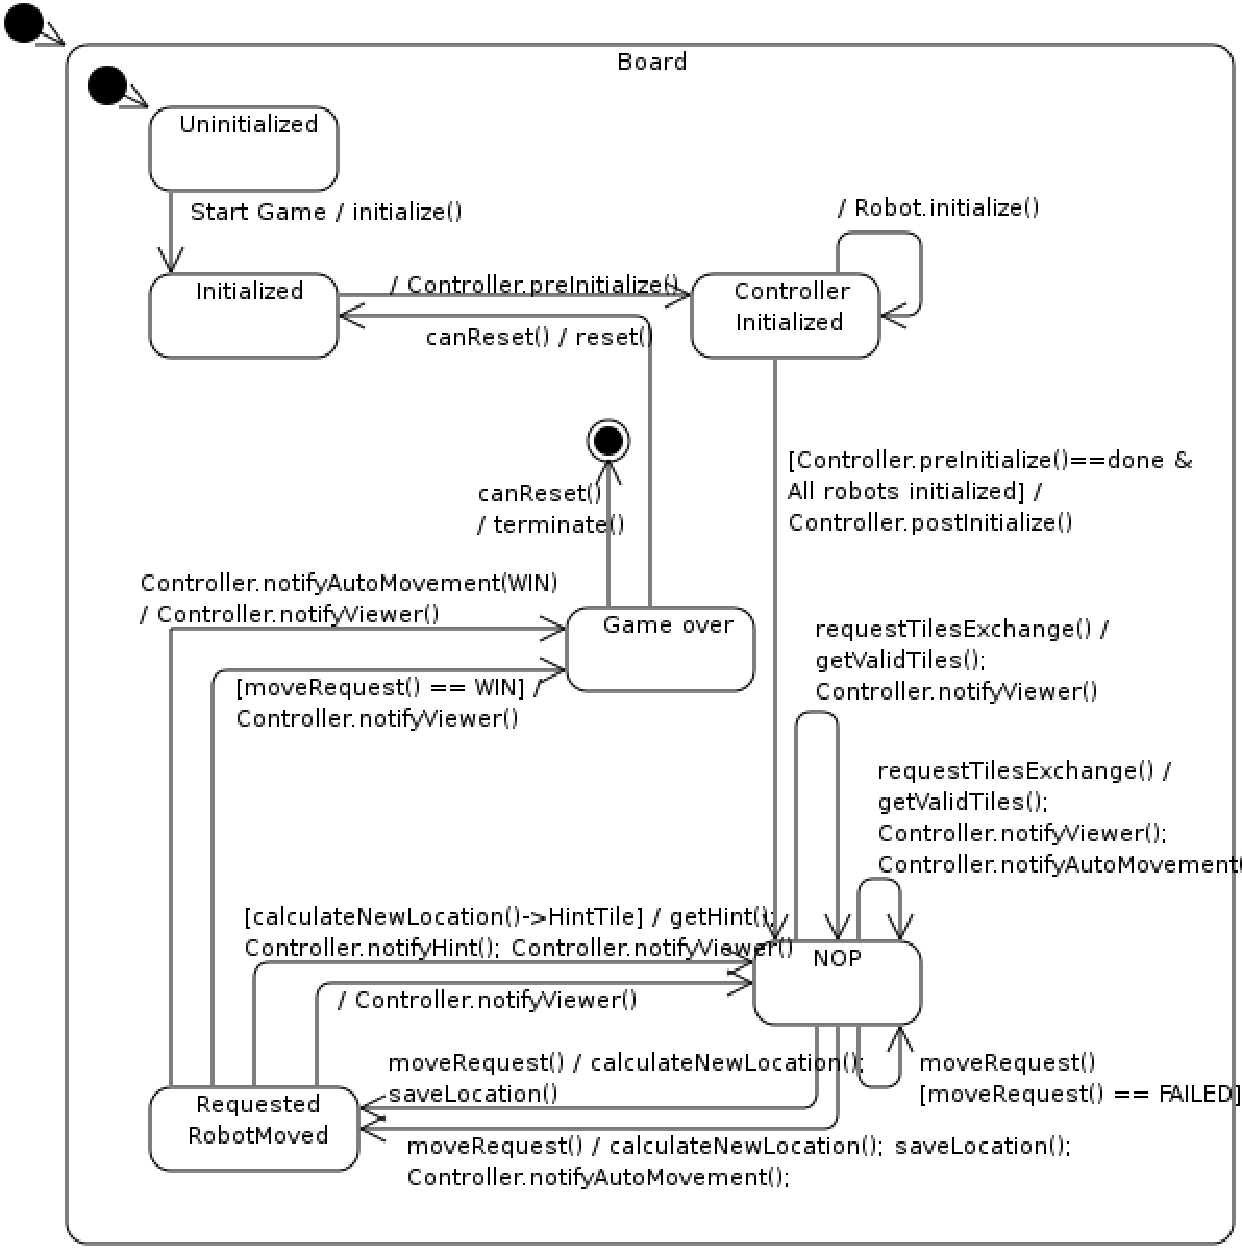
\includegraphics[width=\linewidth]{statecharts/board.pdf}

	\subsubsection{Controller}
	The controller initializes in two phases, the first phase is the preInitialize() during which it waits for other classes to initialize. The second phase is the postInitialize() function, when the controller is in this phase, it knows that all the other classes have been initialized and is aware of the state of all the classes and goes to the NOP state from which most actions take place.\\
If a robot requests a move, the controller goes in to the MoveRequested state, after that it goes to a new state depending on the response of the board. If the board response equals FAILED, the robot is not moved and the controller goes back to the NOP state. If the board response equals WIN the controller will send a notifyStateChange() and notifyGameOver() to let it know that the board has changed and the game has ended, it will also send a terminate() function to the other classes because the game is over and terminate itself in the end. If the board response equals SUCCES the controller switches 2 tiles using Board.requestTilesExchange() and sends a Robot.notifyHint() if needed, it will go to the TilesSwitched state and call the Viewer.notifyStateChange() either way.\\
After the 2 tiles are switched the robots that have been moved by this tileswitch are notified via the Robot.notifyAutoMovement() and the viewer receives an update via the Viewer.notifyStateChange().\\


	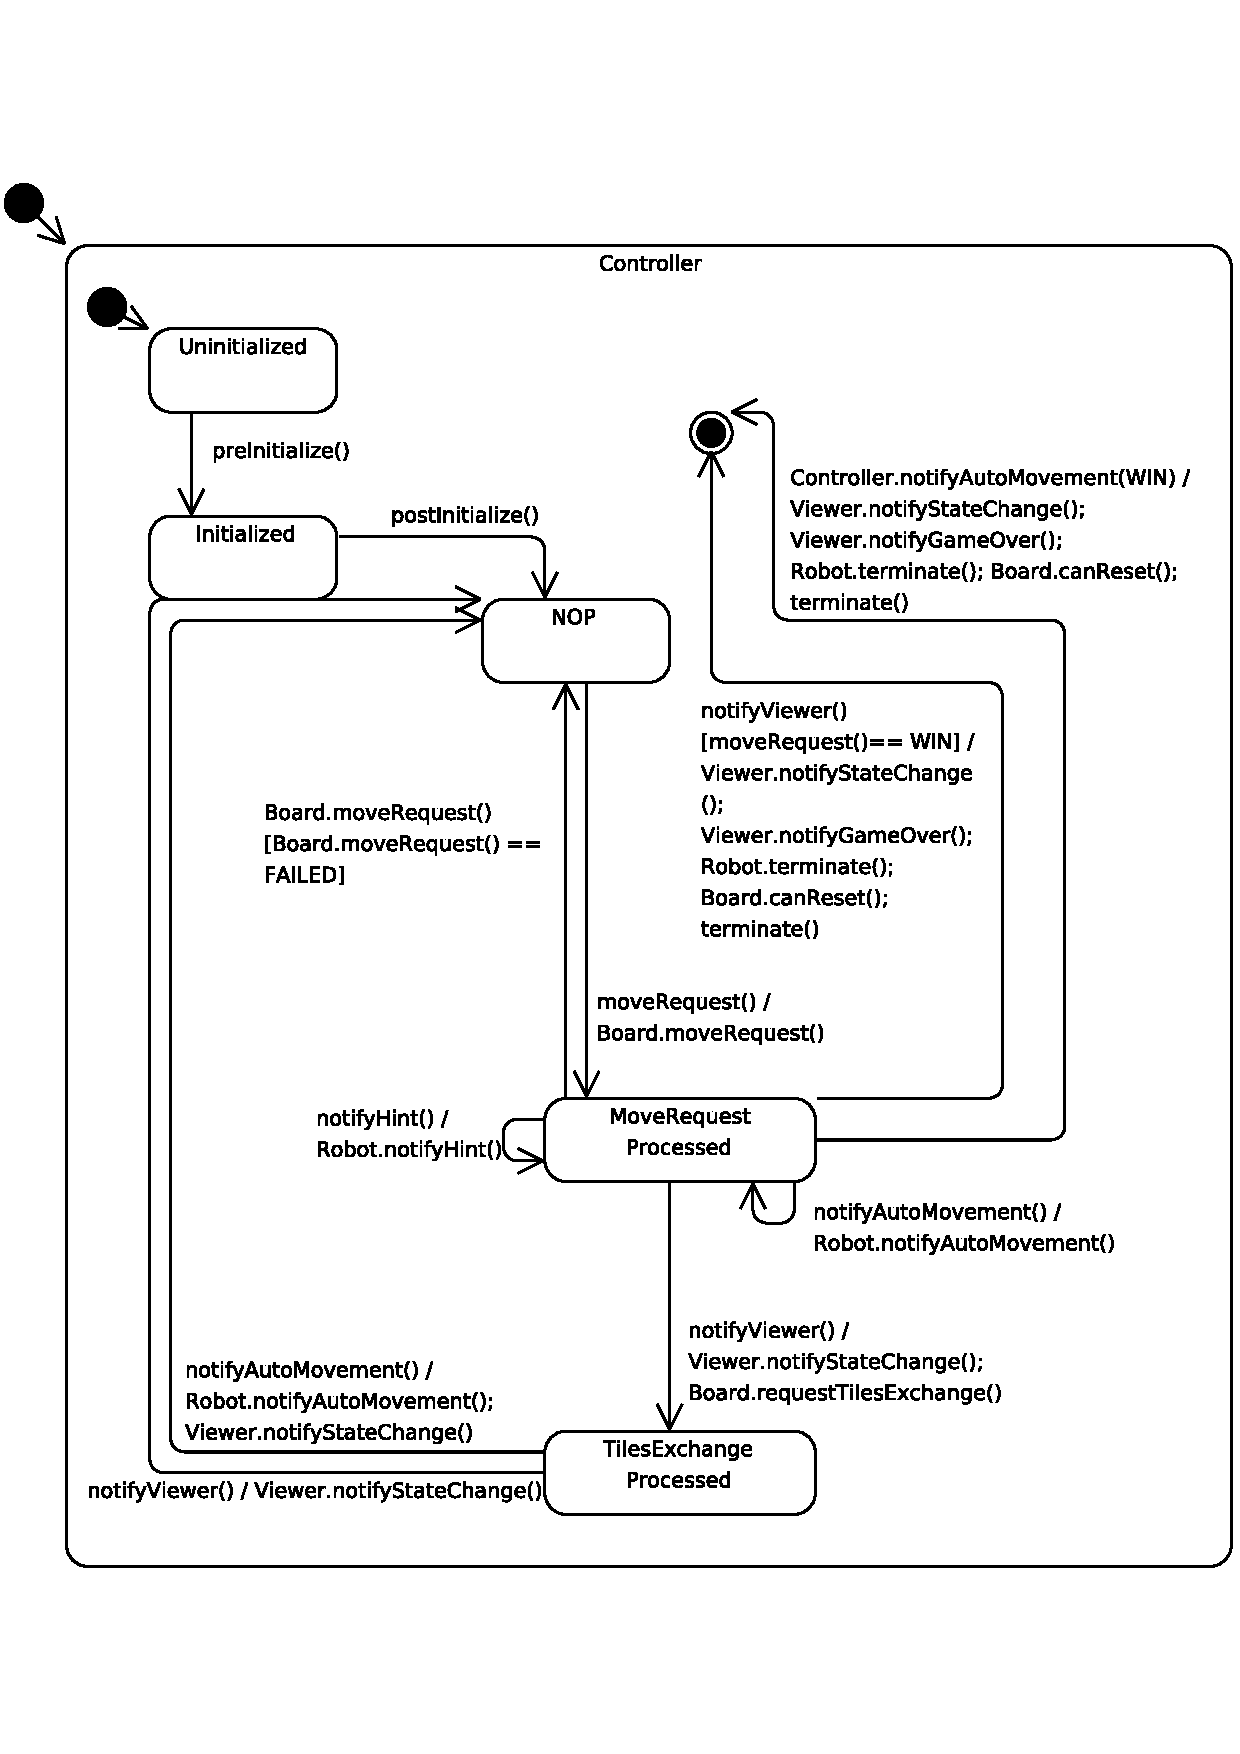
\includegraphics[width=\linewidth]{statecharts/controller.pdf}

	\subsubsection{Viewer}
	After being initialized the viewer comes in the NOP state, which means that it isn't doing anything, but it receives updates from the controller every now and then.... If the board has been changed the function updateView() is called to make the changes visible, it also sends out a notifyStateChange() to let the other classes know the state has changed. The viewer is removed when the game is over, but because there can be multiple viewers, it can also decide to remove itself.
	
	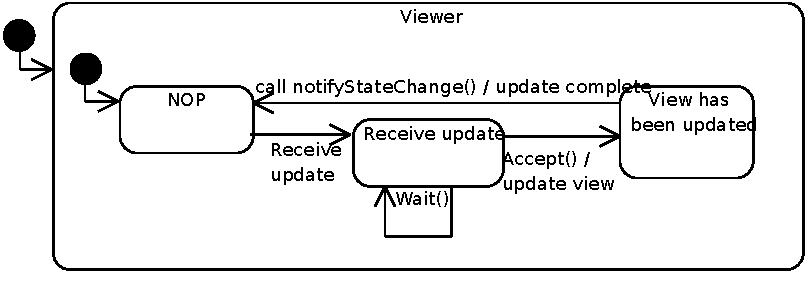
\includegraphics[width=\linewidth]{statecharts/view.pdf}

	\subsubsection{Robot}
	The robot class gets initialized by the controller, it starts at a randomly picked spot, which can be a normal tile, a hint tile or a conveyer tile. The robot receives a notifyAutomovement() every time it gets moved, this can happen in two ways: the robot steps on a conveyer belt or the robot gets moved via a tileswitch. Whenever a robot is on a tile It can request a move which can result in three ways: success, failed or win. If a move request is a success, the move is made, if a move request is a failure, the move is not made because the desired path of the moved Is blocked, if a move request results in a win it means that the robot has reached its hometile the game ends and this robot has won. When another robot wins this robot gets a terminate request from the controller and the game is over. The robot can also encounter hint tiles which point the robot to the location of its hometile.
	
	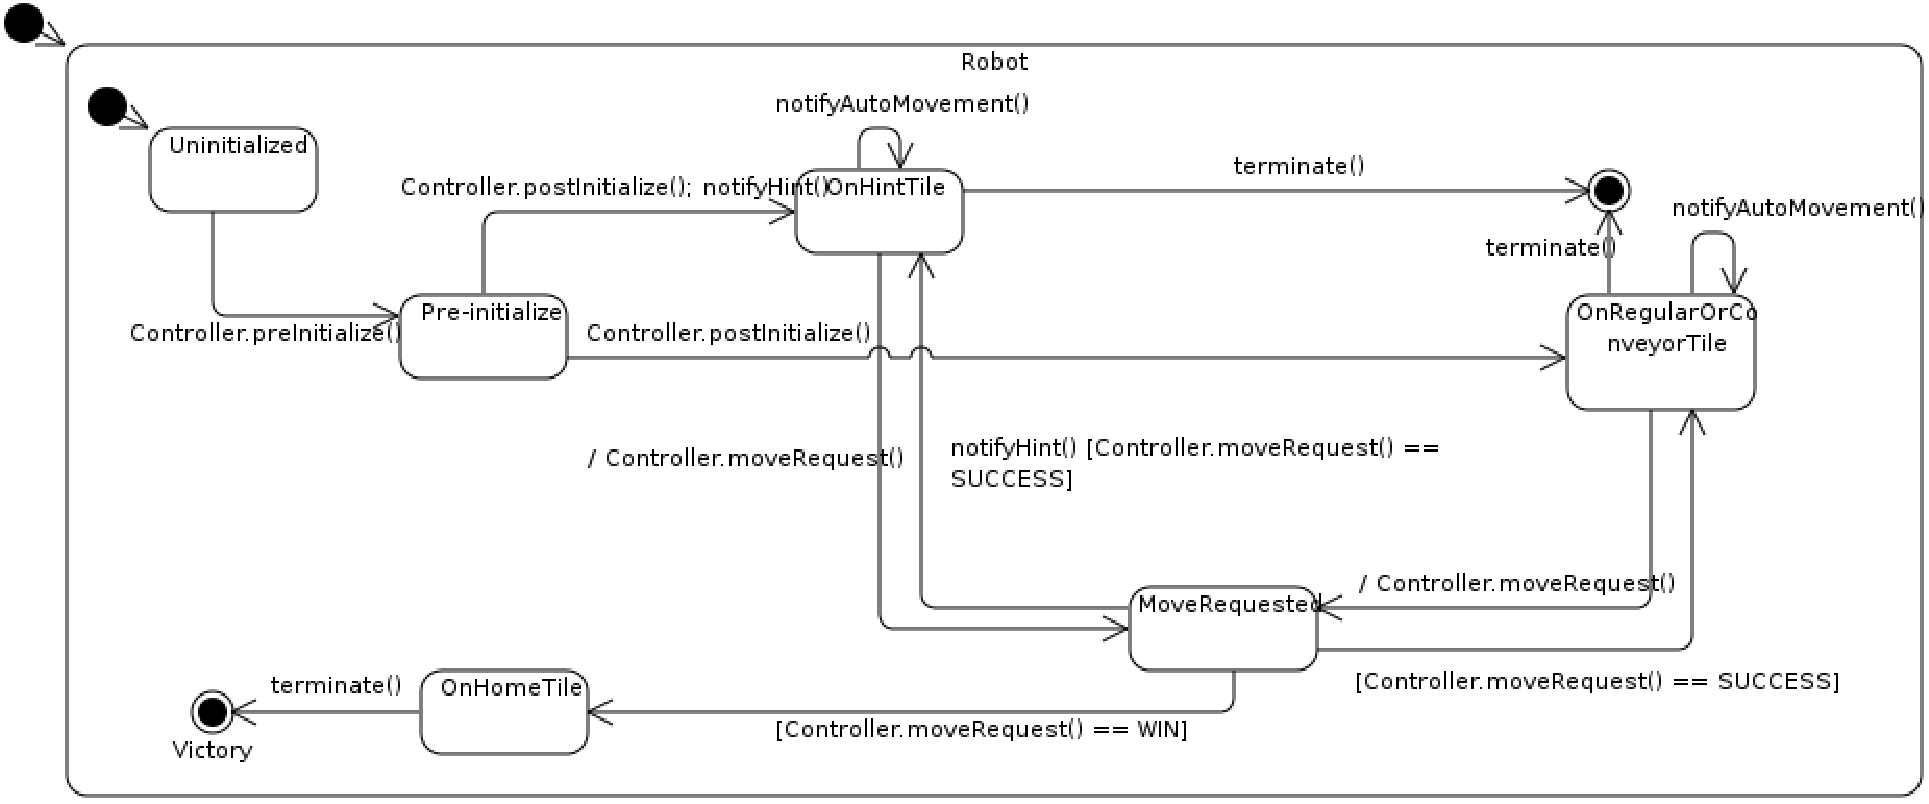
\includegraphics[width=\linewidth]{statecharts/robot.pdf}

\subsection{System level}
	The following graph is our system level state chart, which contains all our class level state charts and gives an overview of the complete system. Although this state chart is mostly trivial, it gives a more complete view of the entire system, thus it is shown below.

	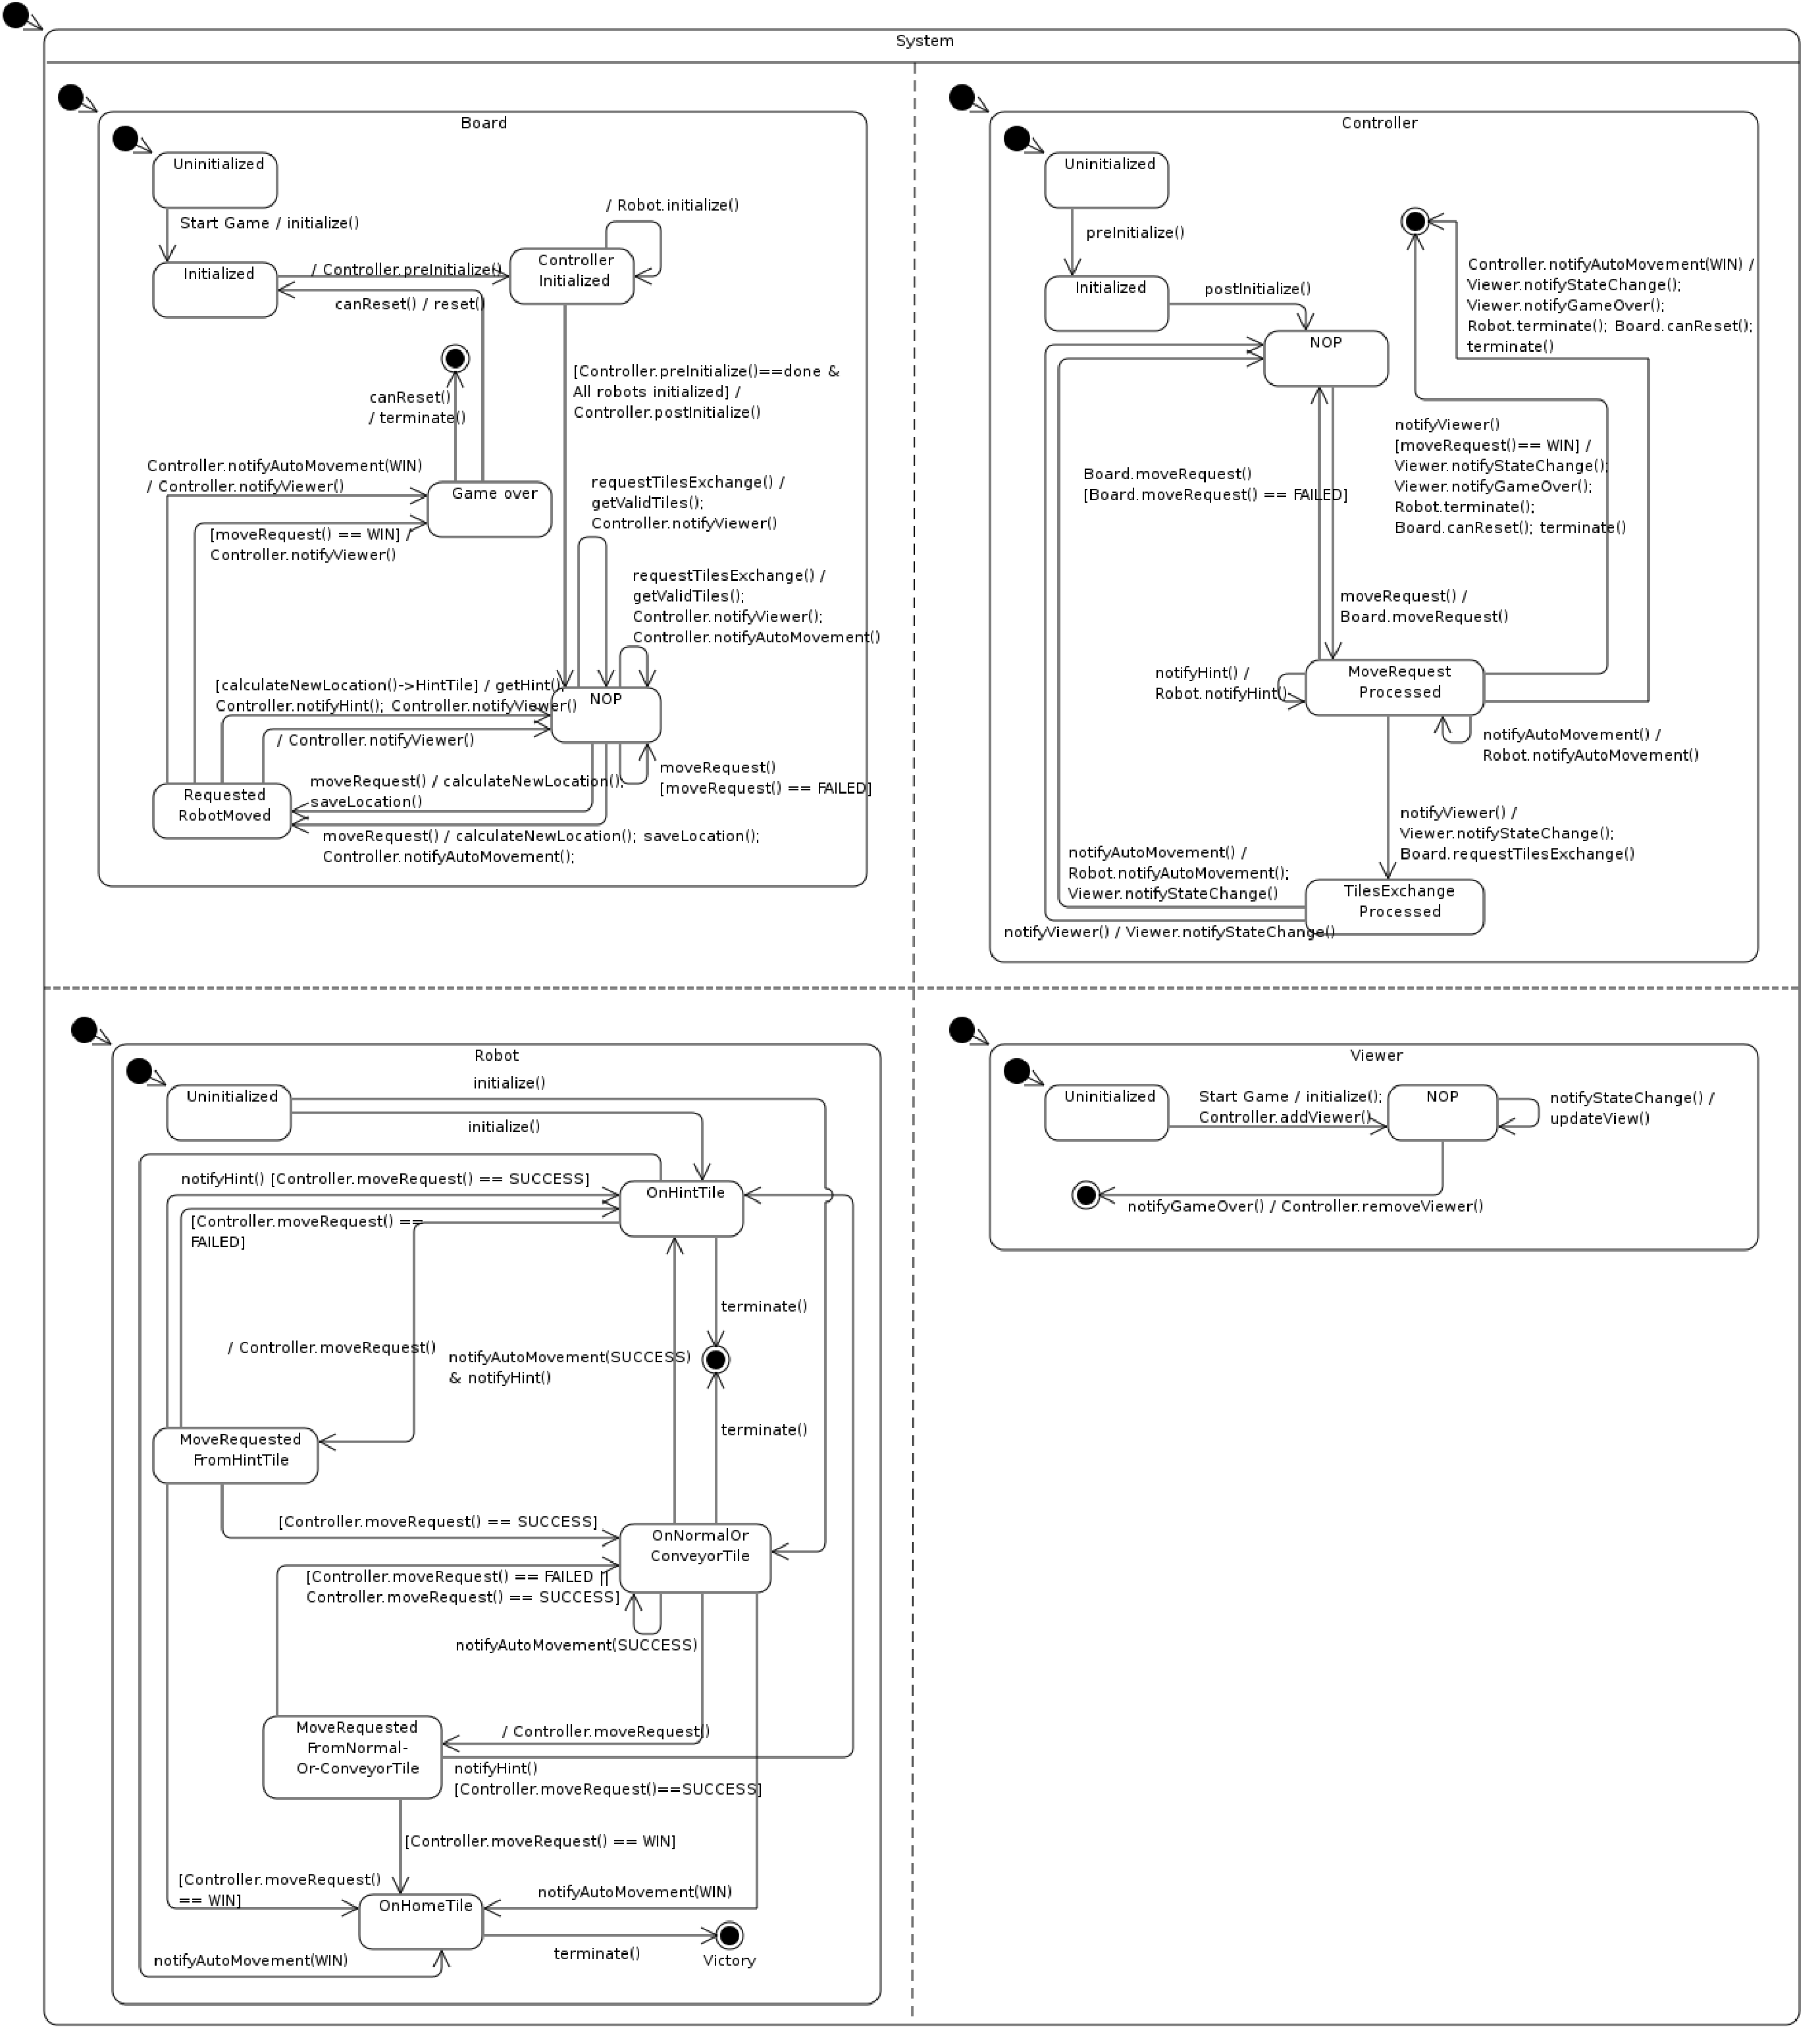
\includegraphics[width=\linewidth]{statecharts/system.pdf}

	

	\newpage

	\section{Z-specification}
	In this section, the formal specification that we are going to use to implement this project is given.

The specification is written in Object-Z, an extension of the Z language.

\subsection{Basic Axiomatic definitions}
We define several attributes that we will use in later definitions in our Z schemas. Since some returned objects in our class diagram may contain null values, we have defined it as a separate set. \\
In our class diagram, we use several enumerators: Hint, BoardResponse and Rotation. Below, we have given the Z specification of these enumerators.

\begin{axdef}
Rotation == \{0, 90, 180, 270\}
\end{axdef}

\begin{axdef}
BoardResponse == \{FAILED, SUCCESS, WIN\}
\end{axdef}

\begin{axdef}
Hint == \{NORTH, EAST, SOUTH, WEST, NORTH\_EAST, \\ \t1 SOUTH\_EAST, SOUTH\_WEST, NORTH\_WEST\}
\end{axdef}

\subsection{Classes}
We distinguish between two types of coordinates: absolute coordinates and relative coordinates. The absolute coordinates describe the coordinates of individual tiles on the Board; these coordinates have an x- and y-value, which are both natural numbers. The relative coordinates are used by Robots to make a move request; the relative coordinates also have an x- and y-value, but these numbers are integers. Since the move requests are communicated to the Board, the Board itself will determine the absolute coordinates that belong to these relative coordinates.

\begin{class}{Null}
\upharpoonright (selfRef) \\
\begin{classcom}
This is a class representing nothing.
\end{classcom} \\
\begin{schema}{selfRef}
output! : Null
\where
output! = self
\end{schema}
\end{class}

\begin{class}{AbsoluteCoord}
\upharpoonright (x, y, BoardWith, BoardHeight) \\
\begin{axdef}
BoardWith : \nat
\end{axdef} \\
\begin{axdef}
BoardHeight : \nat
\end{axdef} \\
\begin{state}
x : \nat \cup \{0\} \\
y : \nat \cup \{0\}
\where
x < BoardWidth \\
y < BoardHeight
\end{state}
\end{class}

\begin{class}{RelativeCoord}
\upharpoonright (x, y) \\
\begin{state}
x : \num \\
y : \num
\end{state}
\end{class}

\begin{classcom}
Calculate the absolute coordinate from an absolute coordinate and a relative coordinate, taking the height / width of the bord into account.
\end{classcom} \\
\begin{axdef}
addAbtoRel == (AbsoluteCoord \cross RelativeCoord) \rightarrow (AbsoluteCoord \union Null)
\where
\forall (a,b) : AbsoluteCoord \cross RelativeCoord | \\ \t1
\IF (0 <= a.x + b.x < BoardWidth \\ \t2
0 <= a.x + b.x < BoardHeigth) \\ \t1
\THEN
addAbtoRel(a,b).x = a.x + b.x \\ \t2
addAbtoRel(a,b).y = a.y + b.y \\ \t1
\ELSE addAbtoRel(a,b) = Null.selfRef
\end{axdef}

Tile class has five specializations: NormalTile, HomeTile, HintTile, ConveyerTile and BrokenRobotTile. A Tile has a type, which is either of the above specializations, and a field 'occupier', which describes the robot that currently occupies the tile. Note that a tile does not necessarily have to be occupied by a robot, so occupies can also be null. All the specializations of Tile inherit the characteristics of Tile.
\begin{class}{Tile}
\upharpoonright (type, occupier) \\
\begin{state}
type : \{NormalTile, HomeTile, ConveyorTile, \\ \t1 BrokenRobotTile, HintTile\} \\
occupier : Robot \cup Null
\end{state} \\
\begin{classcom}
clearTile is a help-method that clears the occupies variable of a Tile.
\end{classcom} \\
\begin{schema}{clear}
\Delta (occupier) \\
\where
occupier' = Null.selfRef
\end{schema} \\
\begin{classcom}
put is a help-method that takes a robot as input-variable and sets the occupies-variable of a Tile to this robot.
\end{classcom}\\
\begin{schema}{put}
\Delta (occupier) \\
input? : Robot
\where
occupier' = input?
\end{schema}
\end{class}

\begin{class}{NormalTile}
Tile
\end{class}

\begin{class}{HintTile}
Tile
\end{class}

\begin{class}{BrokenRobotTile}
Tile
\end{class}

\begin{class}{HomeTile}
Tile \\
\upharpoonright (target) \\
\begin{classcom}
A HomeTile always belongs to one specific Robot, the target robot.
\end{classcom} \\
\begin{state}
target : Robot
\end{state}
\end{class}

\begin{class}{ConveyorTile}
Tile \\
\upharpoonright (rotation) \\
\begin{classcom}
A ConveyerTile has a certain rotation, which influences the direction in which a robot is transported.
\end{classcom} \\
\begin{state}
rotation : Rotation
\end{state}
\end{class}

The Board class maintains several invariants and has a variety of methods, since it is one of the major components of the game.

\begin{class}{Board}
\upharpoonright (tiles, robots) \\
\begin{state}
tiles : \power (AbsoluteCoord \fun Tile) \\
robots : \power (Robot \fun Rotation)
\where
\forall r : robots | \exists c : \dom tiles @  \\ \t1 tiles(c).type = HomeTile \wedge tiles(c).target = r \wedge \\ \t1
\exists d : \dom tiles @ d.occupier = r \wedge Reachable(c, d)
\end{state} \\
\begin{schema}{Occupied}
coord? : AbsoluteCoord \\
output! : \bool
\where
output! = (tiles(coord).type = BrokenRobotTile \; \; \vee \\ \t1
tiles(coord).occupier \not = Null
\end{schema} \\
\begin{schema}{ConveyorUnitDest}
coordA? : AbsoluteCoord \\
coordB? : AbsoluteCoord \\
output! : \bool
\where
output! = \neg Occupied(coordB) \\ \t1
        tiles(input?).type = ConveyorTile \\ \t1
        tiles(input?).rotation = 0 \Rightarrow \\ \t2 input?.x = output!.x + 1 \wedge input?.y = output!.y \\ \t1
        tiles(input?).rotation = 90 \Rightarrow \\ \t2 input?.x = output!.x \wedge input?.y = output!.y - 1 \\ \t1
        tiles(input?).rotation = 180 \Rightarrow \\ \t2 input?.x = output!.x - 1 \wedge input?.y = output!.y \\ \t1
        tiles(input?).rotation = 270 \Rightarrow \\ \t2 input?.x = output!.x \wedge input?.y = output!.y + 1) \\ \t1
\end{schema} \\
\znewpage
\begin{schema}{ConveyorDest}
input? : AbsoluteCoord \\
output! : AbsoluteCoord
\where
\IF ConveyorUnitDest(input?, output!) \\
\THEN output! = input? \\
\ELSE output! = \exists c : AbsoluteCoord | \\ \t2 ConveyorUnitDest(input?, c) \\ \t2 ConveyorDest(c, output!)
\end{schema} \\
\begin{schema}{Adjacent}
coordA? : AbsoluteCoord \\
coordB? : AbsoluteCoord \\
output! : \bool
\where
output! = |\!coordA.x - coordB.x\!| + \\ \t1 |\!coordA.y - coordB.y\!| = 1 \\ \t1
\neg Occupied(coordB)
\end{schema} \\
\begin{schema}{Reachable}
coordA? : AbsoluteCoord \\
coordB? : AbsoluteCoord \\
output! : \bool
\where
output! = ConveyorDest(coordA?) = coordB? \: \vee \\ \t1 (\exists c : AbsoluteCoord | \\ \t2 Adjacent(ConveyorDest(coordA?), c) \: \wedge \\ \t2 ConveyorDest(c) = output!) \: \vee \\ \t1
(\exists c,d : AbsoluteCoord | \\ \t2 Adjacent(ConveyorDest(coordA?), c) \: \wedge \\ \t2 ConveyorDest(c) = d \: \wedge \\ \t2 Reachable(d, output!))
\end{schema} \\
\znewpage
\begin{classcom}
Initialize is called from the outside world, when a new game has to be started. Note that the tiles and robots in this method are read from an input file. After the tiles and robots have been initiated, the Board pre-initializes the Controller and initializes all the robots. Finally, the Board post-initializes the Controller with the initialized Robots and the Board.
\end{classcom} \\
\begin{schema}{Initialize}
\Delta (tiles, robots, controller)
\where
tiles' = createTiles \\
robots' = createRobots \\
controller'.preInitialize \\
\forall r : \dom Robots | r.initialize(controller)
\end{schema} \\
\begin{classcom}
The method below creates a set of robots from a file. This is not further specified.
\end{classcom} \\
\begin{schema}{createRobots}
output! : \power (Robot \fun Rotation)
\end{schema} \\
\begin{classcom}
The method below creates a set of tiles from a file. This is not further specified.
\end{classcom} \\
\begin{schema}{createTiles}
output! : \power (AbsoluteCoord \fun Tile)
\end{schema} \\
\begin{classcom}
CanReset is used by the Controller to let the Board know that the game has ended and that the Board can reset. The Board can reset whenever there is HomeTile on the Board that is occupied by the target robot.
\end{classcom} \\
\begin{schema}{canReset}
\where
(\exists t : Tile | t.type = HomeTile \\ \t1
t.occupier = t.target) \Rightarrow board.reset
\end{schema} \\
\begin{classcom}
When the Board resets itself, the tiles, the controller and the robots are deleted.
\end{classcom} \\
\begin{schema}{reset}
\Delta (tiles, robots)
\where
tiles' = Null.selfRef \\
robots' = Null.selfRef \\
controller' = Null.selfRef
\end{schema} \\
\znewpage
\begin{classcom}
We make a snapshot by copying all the tiles and adding a mapping (same as for the original board). Next, with this snapshot the view can display the board.
\end{classcom} \\
\begin{schema}{requestSnapShot}
boardSnapshot : BoardSnapShot \\
output! : BoardSnapshot
\where
\forall (c,t) : tiles |  \\ \t1
\exists (d,u) : boardSnapshot | c = d \: \wedge \\ \t2 t \not = u \wedge t.type = u.type \: \wedge \\ \t2 t.occupier = u.occupier \: \wedge \\ \t2 t.type = HomeTile \Rightarrow t.target = u.target \: \wedge \\ \t2 t.type = ConveyorTile \Rightarrow t.rotation = u.rotation \\
output! = boardSnapshot
\end{schema} \\
\begin{classcom}
GetHint is used by the Board to generate a hint. It takes the robot that requested a move as input-parameter. It checks where the HomeTile of the robot is and according to that gives the appropiate hint.
\end{classcom} \\
\begin{schema}{getHint}
robot? : Robot \\
output!: Hint
\where
\exists t, t1: \ran tiles | t.occupier = robot? @\\ \t1
t1.type = HomeTile @ t1.target = robot? \\ \t1
\exists coord, coord1: AbsoluteCoord | tiles(coord) = t \\ \t2
\IF coord.x = coord1.x \\ \t2
\THEN \\ \t3
\IF coord.y < coord1.y \\ \t3
\THEN output! = SOUTH \\ \t3
\ELSE output! = NORTH \\ \t2
\ELSE \\ \t3
\IF coord.x > coord1.x \\ \t3
\THEN output! = getHintLeft(coord , coord1) \\ \t3
\ELSE output! = getHintRight(coord, coord1)
\end{schema} \\
\znewpage
\begin{classcom}
This method is a sub method of getHint, used to deal with HomeTile to the left of the robot.
\end{classcom} \\
\begin{schema}{getHintLeft}
absCoord? : AbsoluteCoord \\
absCoord1? : AbsoluteCoord \\
output! : Hint
\where
\IF absCoord?.y = absCoord1?.y \\
\THEN output! = WEST \\
\ELSE \\ \t1
\IF absCoord?.y < absCoord1.y \\ \t1
\THEN \exists hint: \{SOUTH, WEST, SOUTH\_WEST\} | \\ \t3 output! = hint \\ \t1
\ELSE \exists hint: \{NORTH, WEST, WEST\_NORTH\} | \\ \t3 output! = hint
\end{schema}\\
\begin{classcom}
This method is a sub method of getHint, used to deal with HomeTile to the right of the robot.
\end{classcom} \\
\begin{schema}{getHintRight}
absCoord? : AbsoluteCoord \\
absCoord1? : AbsoluteCoord \\
output! : Hint
\where
\IF absCoord?.y = absCoord1?.y \\
\THEN output! = EAST \\
\ELSE \\ \t1
\IF absCoord?.y < absCoord1.y \\ \t1
\THEN \exists hint: \{SOUTH, EAST, EAST\_SOUTH\} | \\ \t3 output! = hint \\ \t1
\ELSE \exists hint: \{NORTH, EAST, NORTH\_EAST\} | \\ \t3 output! = hint
\end{schema} \\
\znewpage
\begin{classcom}
getValidTiles corresponds to the private method in Board. The output is a pair of two valid tiles. A tile is valid for an exchange if it is not a HomeTile or a HintTile. Off course, the invariant also holds for this function.
\end{classcom} \\
\begin{schema}{getValidTiles}
output! : (Tile \cross Tile)
\where
\exists t,t1: Tile | t \not = t1  @ \\ \t1
t.type \not = HomeTile \\ \t1
t.type \not = HintTile \\ \t1
t1.type \not = HomeTile \\ \t1
t1.type \not = HintTile \implies \\ \t1
output! = (t \cross t1)
\end{schema} \\
\begin{classcom}
Method to exchange the positions of two tiles on the board. These tiles should be valid. If a robot is on one of the tiles, it moves along.
\end{classcom} \\
\begin{schema}{requestTilesExchange}
\Delta (tiles)
output! : ({Robot \union Null} \cross {Robot \union Null}) \\
(tile, tile1) : Tile \cross Tile
\where
(tile, tile1)  = getValidTile \\
\exists abCoord, abCoord1 : AbsoluteCoord | tiles(abCoord) = tile \\ \t1
tiles(abCoord1) = tile1 \implies \\ \t2
tiles(abCoord)' = tile1 \\ \t2
tiles(abCoord1)' = tile \\ \t2
\exists n : notifyView \\ \t2
\exists r : Robot | tile.occupier = r \implies \\ \t3
\exists rotation : Rotation | robots(r)' = rotation \\ \t3
\exists n : notifyStateChange | n.input? = r \\ \t2
\exists r1 : Robot | tile1.occupier = r \implies \\ \t3
\exists rotation1 : Rotation | robots(r1)' = rotation1 \\ \t3
\exists n1: notifyStateChange | n1.input? = r1 \\ \t2
\IF tile.occupier = Null.selfRef \\ \t3
tile1.occupier \not = Null.selfRef\\ \t2
\THEN \exists m : moveConveyorSwitch | \\ \t3 \t1 m.absoluteCoord? = abCoord1 \\ \t3
\IF tile1.occupier = Null.selfRef \\ \t3
tile.occupier \not = Null.selfRef \\ \t2
\THEN \exists m : moveConveyorSwitch | \\ \t3 \t1 m.absoluteCoord? = abCoord1
\end{schema} \\
\znewpage
\begin{classcom}
Method to deal with the fact that a robot is part of a tile exchange.
\end{classcom} \\
\begin{schema}{specialExchange}
\Delta (robots)
tile? : Tile
\where
\exists r : Robot | tile.occupier = r \implies \\ \t1
controller.notifyAutoMovement(r) \\ \t1
\exists rotation : Rotation | robots(r)' = rotation
\end{schema} \\
\begin{classcom}
Make sure that a robot on a conveyor belt is moved to the proper tile.
\end{classcom} \\
\begin{schema}{moveConveyorSwitch}
absoluteCoord? : AbsoluteCoord \\
\where
moveConveyorSwitchSub(absoluteCoord?, 0,1) \\
moveConveyorSwitchSub(absoluteCoord?, 1,0) \\
moveConveyorSwitchSub(absoluteCoord?, 0,-1) \\
moveConveyorSwitchSub(absoluteCoord?, -1,0) \\
\end{schema}\\
\begin{classcom}
Subfunction of moveConveyorSwitch, does the actual calculation of the placement of the robot.
\end{classcom} \\
\begin{schema}{moveConveyorSwitchSub}
absoluteCoord? : AbsoluteCoord \\
x? : int \\
y? : int \\
relCoord : RelativeCoord
\where
relCoord.x = x? \\
relCoord.y = y? \\
\IF tiles(addAbtoRel(absoluteCoord?, relCoord)).type = ConveyorTile \\ \t1
tiles(absoluteCoord?).occupier = Null \\ \t1
\exists r : Robot | \\ \t2 tiles(addAbtoRel(absoluteCoord?, relCoord)).occupier = r \\
\THEN moveConveyorSwitch(addAbtoRel(absoluteCoord?, relCoord)\\ \t1
saveLocation(addAbtoRel(absoluteCoord?, relCoord), r)
\end{schema} \\
\znewpage
\begin{classcom}
This functions deals with the moveRequest of the controller
\end{classcom} \\
\begin{schema}{moveRequest}
localCoords? : RelativeCoord \\
robot? : Robot \\
rotation? : Rotation \\
absoluteCoord : AbsoluteCoord \\
output! : BoardResponse
\where
\IF rotation? \not = 0 \\
\THEN response! = moveRotate(localCoords?, robot?, rotation?) \\
\ELSE response! = moveWalk(localCoords?, robot?)
\end{schema} \\
\begin{classcom}
Used to deal with rotations a robot wants to make.
\end{classcom} \\
\begin{schema}{moveRotate}
localCoords? : RelativeCoord \\
robot? : Robot \\
rotation? : Rotation \\
output! : BoardResponse
\where
\IF localCoords.x = 0 \\ \t1
localCoords.y = 0 \\ \t1
 \exists r : robot?.rule.possibleRotations | r = rotation?\\
\THEN output! = SUCCESS \\ \t1
robots(robot?) = (robots(robot?) + rotation?) \mod 360 \\
\ELSE output! = FAILED
\end{schema} \\
\begin{classcom}
Used to deal with other movements a robot wants to make.
\end{classcom} \\
\begin{schema}{moveWalk}
localCoords? : RelativeCoord \\
robot? : Robot \\
output! : BoardResponse
\where
\IF robot?.rule.possibleMoves(localCoords?, robots(robot?)) = \\ \t1
possiblePath(robot?) \wedge rotation? = 0 \\
\THEN absoluteCoord = calculateNewLocation(localCoords?, robot?)\\ \t1
\IF absoluteCoord = Null \\ \t1
\THEN output! = FAILED \\ \t1
\ELSE output! = checkTile(absoluteCoord?, robot?)\\ \t2
\ELSE output! = FAILED
\end{schema} \\
\znewpage
\begin{classcom}
Subfunction of moveWalk, used to check on which tile the robot will end and gives the proper response.
\end{classcom} \\
\begin{schema}{checkTile}
absoluteCoord? : AbsoluteCoord \\
robot? : Robot \\
output! : BoardResponse
\where
saveLocation(absoluteCoord?, robot?) \\
\IF tiles(absoluteCoord?).type = HomeTile \\ \t1
tiles(absoluteCoord?).target = robot? \\
\THEN output! = WIN \\ \
\ELSE  \\ \t1
\IF tiles(absoluteCoord?).type = ConveyorTile \\ \t1
\THEN controller.notifyAutomovement(robot?) \\ \t1
\IF tiles(absoluteCoord?).type = HintTile \\ \t1
\THEN controller.notifyHint(Board.getHint(robot?), robot?) \\ \t1
output! = SUCCESS
\end{schema} \\
\begin{classcom}
saveLocation corresponds to the private method in Board. It has two input-variables: absCoords, which is an absolute coordinate and robot, which is the robot that has been moved.  If we want to save the new location of the robot, the Tile that becomes the new location must be empty. The help-method put is used to place the robot on the empty Tile. After the location has been saved, the viewer is notified of the robot's location change, so it can redraw the Board.
\end{classcom} \\
\begin{schema}{saveLocation}
absCoords? : AbsoluteCoord \\
robot? : Robot
\where
\exists t : Tile | t.occupier = robot? \wedge t.clear\\
tiles(absCoords?).put(robot) \\
viewer.notifyView
\end{schema}
\znewpage
\begin{classcom}
Function to calculate the location of a robot according to it's path.
\end{classcom}\\
\begin{schema}{calculateNewLocation}
localCoords? : RelativeCoord \\
robot? : Robot \\
absoluteCoord : AbsoluteCoord \\
output! : (AbsoluteCoord \union Null)
\where
\IF checkPath(localCoords?, robot?) \\
\THEN absoluteCoord = firstConveyor(c, path) \\ \t1
\exists s : ConveyorDest | s.input? = absoluteCoord @ \\ \t2
output! = s.output! \\
\ELSE output! = Null.selfRef
\end{schema} \\
\begin{classcom}
Function to check if the path is free (if not, a ConveyorTile should be in front of the obstacle in order to let the path be valid). Calculate new coordinates as well
\end{classcom} \\
\begin{schema}{checkPath}
localCoords? : RelativeCoord \\
robot? : Robot \\
path : seq RelativeCoord \\
absoluteCoord : AbsoluteCoord \\
bool : \bool \\
output! : \bool
\where
bool = false \\
path = robot?.rule.possibleMoves(localCoords? \cross robots(robot?)) \\
\exists (c, t) : tiles | t.occupier = robot? \implies \\ \t1
\forall (int, coord) : path | \\ \t2
((addAbtoRel(c, coord) = Null \vee \\ \t2
(tiles(addAbtoRel(c, coord).type = BrokenRobotTile) \vee \\ \t2
\exists r: Robot | tiles(addAbtoRel(c, coord).occupier = r )\implies \\ \t3
\exists (int1, coord1) : path | int1 < int \\ \t3
tiles(addAbtoRel(c, coord1).type = ConveyorTile \\ \t3
absoluteCoord = addAbtoRel(c, coord1)) \implies \\ \t4
bool = \true \\ \t4
output! = bool
\end{schema} \\
\znewpage
\begin{classcom}
Calculate the first occuring ConveyorTile for a given path.
\end{classcom} \\
\begin{schema}{firstConveyor}
firstConveyor == (AbsoluteCoord \cross seq RelativeCoord) \fun \\ \t1 AbsoluteCoord
\where
\exists absoluteCoord : AbsoluteCoord |  \\ \t1
\exists (int, coord): seq RelativeCoord |  \\ \t2
(tiles(addAbtoRel(absoluteCoord, coord).type = conveyorTile \\ \t2
conveyorInPath(absoluteCoord, (int, coord)) = \\ \t3 addAbtoRel(absoluteCoord, coord)) \implies \\ \t3
\forall (int1, coord1): seq RelativeCoord | \\ \t3
\IF tiles(addAbtoRel(absoluteCoord, coord1).type = conveyorTile \\ \t3
\THEN int <= int1
\end{schema}
\end{class}

A BoardSnapshot is simply a copy of the current state of the board; therefore, the BoardSnapshot maintains a mapping of absolute coordinates to the tiles.
\begin{class}{BoardSnapshot}
\upharpoonright (tiles) \\
\begin{state}
tiles : \power (AbsoluteCoord \fun Tile) \\
\end{state}
\end{class}

A Rule consists of a list of possible moves and a list of possible rotations. The possible moves are described in terms of local coordinates, since a robot does not know its exact location on the board. Since each robot has a certain rotation, possibleMoves maps relative coordinates and rotations to each possible relative coordinate that the robot can move to. The list of possible rotations is simply a list of all rotations.
\begin{class}{Rule}
\upharpoonright (possibleMoves, possibleRotations) \\
\begin{state}
possibleMoves : \power ((RelativeCoord \times Rotation) \psurj \\ \t1 \seq RelativeCoord) \\
possibleRotations : \power Rotation
\end{state} \\
\end{class}

A Robot has knowledge of the Controller and maintains a rule-attribute, describing the ruleset of the Robot.
\begin{class}{Robot}
\upharpoonright (rules) \\
\begin{state}
rules : Rules \\
controller : Controller
hint : Hints
\end{state}\\
\begin{classcom}
The initialize of the Robot uses the parameters controller and rules. The controller-parameter is the initialized Controller; the rules-parameter is the set of rules that determine the possible moves and rotations. In the initialize, all the provided input-values are saved and the list of hints is initially empty, since the Robot has not yet received any hints.
\end{classcom} \\
\begin{schema}{initialize}
\Delta (controller, rules, hint) \\
controller? : Controller \\
rules? : Rules
\where
controller' = controller? \\
rules' = rules? \\
hint' = Null.selfRef
\end{schema}\\
\begin{classcom}
NotifyAutoMovement is used by the Controller to notify that the Robot was moved, because of a conveyor belt. Note that the Robot could be rotated by a conveyor belt, so the list of hints is cleared; the Robot has now no idea where its Home Tile is.
\end{classcom} \\
\begin{schema}{notifyAutoMovement}
\Delta (hint)
\where
hint' = Null.selfRef
\end{schema}\\
\begin{classcom}
NotifyHint is used by the Controller to pass the hint of the Board to the Robot. Since each Robot may store a list with all the hints it has received, the new hint is simply added to the list of hints.
\end{classcom} \\
\begin{schema}{notifyHint}
\Delta (hint) \\
hint? : Hint
\where
hint' = \{hint?\} \union hint
\end{schema}
\end{class}

The Viewer has no knowledge of the Board; every change of the Board must be communicated to the Viewer via the Controller. The variable 'boardChanged' is used as a flag to indicate that the board has changed and the Viewer has not yet updated the view.
\begin{class}{Viewer}
\begin{state}
controller : Controller \\
boardChanged : \bool
\end{state}\\
\begin{classcom}
In initialize, the Viewer attaches itself to the Controller, using the addViewer-method; the viewer parameter in addViewer is this Viewer. ???
\end{classcom} \\
\begin{schema}{initialize}
\Delta (controller)
\where
\exists a : addViewer | a.viewer? = self \implies \\ \t1
a.output! = controller' \\ \t1
boardChanged' = \false
\end{schema}\\
\begin{classcom}
When the game has ended, the Viewer is notified by the Controller via notifyGameOver. The Viewer will now show an animation of fireworks and all robots that have not won the game will explode.
\end{classcom} \\
\begin{schema}{notifyGameOver}
robot? : Robot
\where
Fireworks
\end{schema}\\
\begin{classcom}
With notifyStateChange, the Viewer is notified by the Controller that the Board has changed. The Viewer sets boardChanged to true, to indicate that it has not yet updated the view.
\end{classcom} \\
\begin{schema}{notifyStateChange}
\Delta (boardChanged)
\where
boardChanged' = \true
\end{schema}\\
\znewpage
\begin{classcom}
The updateView-method uses the value of boardChanged to update the view. If this variable is true, then the Viewer requests a new snapshot from the Board, via the Controller, and updates the view. After the update, boardChanged is set to false. If boardChanged is false, then the previous snapshot is still up-to-date and nothing is changed. Note that the variable controller in Viewer never changes here, because it is simply used to request a board snapshot.
\end{classcom} \\
\begin{schema}{updateView}
\Delta (controller, snapShot)
\where
\IF boardChanged = \true \\
\THEN \exists r: requestBoardStatus | output! = snapShot' \\ \t1
boardChanged' = \false \\ \t1
controller' = controller \\
\ELSE snapShot' = snapShot \\ \t1
boardChanged' = \false \\ \t1
controller' = controller
\end{schema}
\end{class}

The controller has knowledge about the Board and the Viewer; it also maintains a list of the robots.
\begin{class}{Controller}
\begin{state}
board : Board \\
robots : \power Robot
viewer : Viewer
\end{state}\\
\begin{classcom}
addViewer corresponds to the public method in Controller. It takes a viewer as an input variable; this is the Viewer that wants to attach itself to the controller. If the Controller did not have a Viewer attached to it yet, then the Controller saves the Viewer and returns itself to the Viewer. The Viewer will then be able to address the controller, for board snapshot requests. If the Controller already had a Viewer attached to it, then the add-request is simply ignored.
\end{classcom} \\
\begin{schema}{addViewer}
\Delta (viewer) \\
viewer? : Viewer \\
output! : Controller
\where
\IF viewer = Null \\
\THEN viewer' = viewer? \\ \t1
output! = self \\
\ELSE output! = Null.selfRef
\end{schema}\\
\begin{classcom}
notifyAutoMovement corresponds to the public method in Controller. It takes the Robot that requested a move as input-parameter. This method is used by the Board to let the Robot know that it has been moved by a conveyor tile. 
\end{classcom} \\
\begin{schema}{notifyAutoMovement}
robot? : Robot
\where
robot?.notifyAutomovement
\end{schema}\\
\znewpage
\begin{classcom}
moveRequest corresponds to the public method in Controller. It takes local coordinates, the Robot that requested the move and a rotation as input-parameters. The Controller forwards the move request of the robot, along with the specified attributes to the Board. If the Board then responds with "WIN", then the Controller must terminate all robots, notify the Viewer that the game has ended and terminate.
\end{classcom} \\
\begin{schema}{moveRequest}
localCoords? : RelativeCoord \\
robot? : Robot \\
rotation? : Rotation \\
ouput! : BoardResponse
\where
\exists m : Board.moveRequest | m.localCoords? = localCoords \\ \t1
m.robot? = robot? \\ \t1
m.rotation? = rotation? \\ \t1
m.output! = output! \\ \t1
\IF output! = WIN \\ \t1
\THEN \forall r : Robot | r.terminate \\ \t2
\exists n : viewer.notifyGameOver | n.robot? = robot? \\ \t2
board.canReset \\ \t2
terminate
\end{schema}\\
\begin{classcom}
Notify the controller of an appropriate hint.
\end{classcom} \\
\begin{schema}{notifyHint}
hint? : Hint \\
robot? : Robot
\where
\exists n : robot.notifyHint | n.hint? = hint?
\end{schema}\\
\begin{classcom}
Notify the viewer that the board has changed.
\end{classcom} \\
\begin{schema}{notifyView}
\where
\exists n : notifyStateChange
\end{schema}
\znewpage
\begin{classcom}
Initialize the controller so that it can be referred to.
\end{classcom} \\
\begin{schema}{preInitialize}
\Delta (board, robots, vieuwer)
\where
board' = Null.selfRef \\
robots' = Null.selfRef \\
viewer' = Null.selfRef
\end{schema}\\
\begin{classcom}
The real initialization of the controller, giving it a board and robots.
\end{classcom} \\
\begin{schema}{postInitialize}
\Delta (board, robots) \\
board? : Board \\
robots? : \power Robot
\where
board' = board \\
robots' = robots?
\end{schema}\\
\begin{classcom}
Remove a viewer (so that eventually, a new one can be added).
\end{classcom} \\
\begin{schema}{removeViewer}
\Delta (viewer, robots, board)
\where
viewer' = Null.selfRef \\
robots' = robots \\
board' = board
\end{schema}\\
\begin{classcom}
Function to get a snapshot of the board.
\end{classcom} \\
\begin{schema}{requestBoardStatus}
output! : BoardSnapShot
\where
\exists r : requestSnapShot | r.output! = output!
\end{schema}
\end{class}

	\newpage

	\section{Conclusion}
	This report has shown how the requested program has been specified by using use cases, message sequence charts, a class diagram, state charts and Z. By the hand of this specification, an implementation has been made which shows the actual fight between the robots.
	\newpage

	\appendix
	\section{Informal specification}
		\label{appendix:informal}
		
\subsection{Inleiding}

Wij willen jullie een spel laten maken wat zich afspeelt in een enorm grote arena, met veel publiek die veel geld betaald hebben om naar dit schouwspel te komen kijken. In deze arena zijn verschillende robots op zoek naar hun eigen thuisvak.

\subsection{Spelregels}

Het spel wordt in de arena gespeeld, waarin een vooraf gedefinieerd eindig spelbord aanwezig is.
Er zijn twee type robots die aan het spel deelnemen. Het eerste type robot kan zich in iedere richting (boven, onder, rechts of links) precies een vakje verplaatsen. Het tweede type robot kan twee soorten zetten doen. De robot kan 1, 2 of 3 hokjes vooruit lopen, of de robot kan draaien, waarbij hij 90, 180 of 270 graden draait. Dit tweede type kan dus in een beurt lopen of draaien, echter niet beide.\\
Er zijn verder vijf type vakjes.
\begin{enumerate}
  \item thuisvakken, als een robot op zijn eigen thuisvak komt heeft hij gewonnen.
  \item hintvakken, als een robot hierop komt krijgt hij een hint waar zijn thuisvak is.
  \item lopende banden, dit zijn vakken waarbij de robot verplaatst wordt, zodra hij hier op staat. Deze lopende banden gaan met een oneindige snelheid, dus zodra een robot op een lopende band stapt wordt hij verplaatst naar een andere plek, voordat hij zelf om een nieuwe verplaatsing kan vragen.
  \item bezette vakken, dit zijn vakken waar al een andere robot staat. Dit kan ook een defecte robot zijn.
  \item normale vakken, dit zijn vakjes waarbij er niets speciaals gebeurt.
\end{enumerate}

\noindent Alle robots in het speelveld zijn op zoek naar hun eigen thuisvak. Iedere robot heeft precies \'{e}\'{e}n thuisvak. Om de robots hierbij een beetje te helpen, zijn er ook verschillende hintvakken, zie figuur 1, (ook hiervan weet de robot de locatie niet, hij moet dus maar met geluk op een hintvak terecht komen).\\
Zodra een robot op een hintvak terecht komt, krijgt de robot een hint over de richting te volgen naar zijn thuisvak. Een hint bestaat puur en alleen uit een richting waar het thuisvak zich bevindt (boven, onder, rechts of links). Als eenzelfde robot een tweede maal op een hintvak terecht komt, kan hij een andere hint krijgen dan de eerste keer.

\begin{figure}
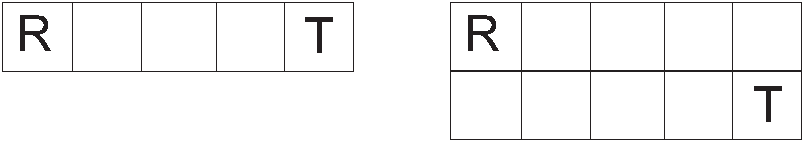
\includegraphics{informal/plaatjes.pdf}
\caption{De robot R staat op een hintvak, en T is het thuisvak. Twee situaties: In de situatie links is de hint $"$rechts$"$. In de situatie rechts zijn er meerdere mogelijkheden, $"$onder$"$, $"$rechts$"$ of $"$rechts en onder$"$.}
\label{hintvakken}
\end{figure}

De locatie van de hintvakken en van de thuisvakken is statisch. Een robot kan hierover dus informatie opslaan. De robot kan geen gegevens over zijn eigen locatie opslaan, aangezien er ook rotatie-transportbanden op het speelveld aanwezig zijn. Iedere transportband verplaatst een robot naar een willekeurige plaats. De robot kan tijdens het transport ook geroteerd zijn. Daarom zijn het ook rotatie-transportbanden. De robot kan dus geen gegevens bewaren over zijn locatie, aangezien de robot verplaatst kan zijn tussen twee beurten. De robots kunnen de transportbanden niet zien. Ze merken door hun ingebouwde gyroscopen wel dat ze bewogen zijn, de gyroscopen zijn echter niet goed genoeg om bij te kunnen houden in welke richting de robot verplaatst is.\\
Zodra een robot op zijn thuisvak aangekomen is, heeft deze robot gewonnen, en kan hij alle andere robots laten ontploffen. Het einde, het ontploffen van alle verliezende robots, is het spektakel waarvoor het publiek gekomen is. Ze barsten na het ontploffen dan ook in juichen uit.

\subsection{Spelbord}

Er is een bord, zodat bijgehouden kan worden welke robot waar staat. Dit bord houdt bij welke robot op welke positie staat. Opdat de spelers met het bord kunnen communiceren moet er een controller zijn. De communicatie geschiedt alleen op de volgende volgorde: het bord ontvangt een request van de speler via de controller. Het bord antwoordt de controller. Deze zal dan weer de speler informeren.\\
Omdat de schoonmakers een beetje lui zijn, staan er op het veld nog kapotte robots uit de vorige gevechten. Het aantal kapotte robots kan vari\"{e}ren van 10 tot 20 procent van het totaal aantal vakjes. Als een robot een verzoek indient om naar een van deze vakjes te gaan, of naar een van de vakjes waarop een andere robot staat, dan wordt dit verzoek afgewezen omdat dit vakje dan al bezet is.\\
Iedere keer dat het spelbord een request toestaat, kiest het bord ook twee vakjes welke omgewisseld worden, als hier een (defecte) robot op staat of als hier een lopende band is, worden de robot en/of lopende band mee verplaatst. Dit houdt in dat ook de ori\"{e}ntatie van de speler en de lopende band verandert kan zijn. Het bord dient er echter wel voor te zorgen dat het altijd mogelijk blijft voor iedere robot om zijn thuisvak te halen. Het bord kan hier alle type vakjes, behalve de hint en thuisvakken verplaatsen. De robot kan dus alleen hier informatie over bijhouden.\\
Als een robot verplaatst wordt, door een lopende band, of doordat er twee vakjes verwisseld worden, geeft het bord dit door aan de controller, die het weer door zal geven aan de robot.\\
Het bord keurt alle zetten af zolang het nog niet ge\"{\i}nitialiseerd is.

\subsection{Speler}

Een speler is een robot die mee doet aan het spelletje. Als de speler zich wil verplaatsen stuurt hij een verzoek tot verplaatsing naar de controller. Het bord krijgt een request van de speler via de controller. Het bord zal beslissen of de zet legitiem is of niet, zo ja dan wordt de speler verplaatst. Aan de controller wordt terug gegeven of de robot is verplaatst of niet, die dit op zijn beurt weer terug geeft aan de speler. \\
Indien een speler op een lopende band komt, maar het einde van de lopende band is geblokkeerd door een andere mogelijk defecte robot, zal de robot op het laatste stukje van de lopende band blijven staan. En kan hij hier wel weer afstappen, als de nieuwe plek tenminste niet ook geblokkeerd is.\\
De spelers kunnen hun zetten gelijktijdig doen, er wordt dus geen volgorde afgedwongen.

\subsection{Viewer}

Om het publiek een beter zicht op het spel te geven hangen er op verschillende plaatsen in de arena beeldschermen. Deze beeldschermen geven een visuele representatie van de staat van de controller en dus ook het bord.

\subsection{Use-Case Scenario's}
Hieronder staan een aantal Use-Cases, zodat jullie kunnen zien hoe de communicatie tijdens het spel verloopt.
\subsubsection*{Robot wil verplaatsen}
\begin{description}
  \item[Pre:] True.
  \item[Trigger:] Robot vraagt toestemming om een stap te doen.
  \item[Guarantee:] Robot is verplaatst.
  \item[Scenario]
    \begin{description}
        \item[]
        \item[Main]
            \begin{enumerate}
              \item[]
              \item De robot zegt tegen de controller dat hij wil verplaatsen.
              \item Controller geeft vraag door aan het bord.
              \item Het bord keurt de vraag goed en verplaatst de robot.
              \item Controller geeft door dat hij verplaatst is.
            \end{enumerate}
        \item[Alternative]
            \begin{itemize}
                \item[]
                \item[3] Het bord keurt de vraag af en de robot blijft staan.
                \item[4] Controller geeft door dat de robot geen toestemming heeft.
            \end{itemize}
    \end{description}
\end{description}
\newpage
\subsubsection*{Robot stapt op lopende band}
\begin{description}
  \item[Pre:] Stap is toegestaan.
  \item[Trigger:] Vakje waar robot op komt is een lopende band.
  \item[Guarantee:] Robot is verplaatst over lopende band.
  \item[Scenario]
    \begin{description}
        \item[]
        \item[Main]
            \begin{enumerate}
              \item[]
              \item Robot stapt op lopende band.
              \item Robot eindigt op vakje na de lopende band.
              \item Robot krijgt te horen dat hij verplaatst is.
            \end{enumerate}
    \end{description}
\end{description}

\subsubsection*{Robot stapt op hintvak}
\begin{description}
  \item[Pre:] Stap is toegestaan.
  \item[Trigger:] Robot komt op een hintvak terecht.
  \item[Guarantee:] Robot krijgt een hint over de positie van zijn thuisvak.
  \item[Scenario]
    \begin{description}
        \item[]
        \item[Main]
            \begin{enumerate}
              \item[]
              \item Robot stapt op hintvak.
              \item Het bord bepaalt aan de hand van de relatieve positie van het thuisvak t.o.v de robot, de hint.
              \item De hint wordt via de controller doorgegeven aan de robot.
            \end{enumerate}
    \end{description}
\end{description}

\subsubsection*{Robot stapt op thuisvak}
\begin{description}
  \item[Pre:] Stap is toegestaan.
  \item[Trigger:] Robot stapt op thuisvak.
  \item[Guarantee:] De verplaatste robot heeft gewonnen.
  \item[Scenario]
    \begin{description}
        \item[]
        \item[Main]
            \begin{enumerate}
              \item[]
              \item Robot stapt op het thuisvak.
	          \item Het bord laat Spelers weten dat de verplaatste robot heeft gewonnen.
            \end{enumerate}
    \end{description}
\end{description}
\newpage
\subsubsection*{Vakjes worden gewisseld}
\begin{description}
  \item[Pre:] True.
  \item[Trigger:] Het bord heeft de request van de robot goedgekeurd.
  \item[Guarantee:] Na het verwisselen van de twee vakjes moet er een mogelijkheid zijn voor alle robots om het thuisvak te kunnen bereiken.
  \item[Scenario]
    \begin{description}
        \item[Main]
            \begin{enumerate}
              \item[]
              \item Er worden twee geldige vakjes gekozen.
              \item De vakjes worden gewisseld.
            \end{enumerate}
        \item[Alternative]
            	\begin{itemize}
			     \item[]
                 \item[2] Als er op een of beide vakjes een lopende band en/of een robot aanwezig is, dan worden alle robots en lopende banden op deze twee vakjes willekeurig een richting op gedraaid (de richting voor en na het draaien kan hetzelfde zijn).
			     \item[3] Het bord geeft via de controller door aan de speler dat de robot verplaatst is.
            	\end{itemize}
    \end{description}
\end{description}

\end{document}
